\documentclass[11pt]{article}
\usepackage[margin=1in]{geometry}
\usepackage{graphicx} % Required for inserting images
\usepackage{amsmath,amssymb,amsthm}
\usepackage{booktabs}
\usepackage{array}
\usepackage[section]{placeins}
\usepackage{pgfplots}
\pgfplotsset{compat=1.17}
\usepackage[hidelinks]{hyperref}

\newtheorem{theorem}{Theorem}[section]
\newtheorem{proposition}[theorem]{Proposition}
\newtheorem{lemma}[theorem]{Lemma}
\newtheorem{conjecture}[theorem]{Conjecture}
\theoremstyle{definition}
\newtheorem{definition}[theorem]{Definition}
\newtheorem{example}[theorem]{Example}
\theoremstyle{remark}
\newtheorem{remark}[theorem]{Remark}

\newcommand{\F}{F}
\newcommand{\nc}[1]{\langle\!\langle #1 \rangle\!\rangle}
\newcommand{\pres}[2]{\langle #1 \mid #2 \rangle}
\newcommand{\Aut}{\operatorname{Aut}}
\newcommand{\rot}{\operatorname{rot}}
\newcommand{\Sol}{\mathcal{S}}
\newcommand{\Orc}{\mathcal{O}}
\newcommand{\Fix}{\mathcal{F}}
\newcommand{\W}{\mathcal{W}}
\newcommand{\MS}{\mathrm{MS}}
\newcommand{\SMK}{\mathrm{S20\_MK2}}

\title{Stable AC-personal}
\author{Avigya Paudel}
\date{October 2026}

\begin{document}

\maketitle

\paragraph{Notation.} Let $X=\{x_1,\dots,x_n\}$ and let $\F(X)$ be the free group on $X$. A word over
$X^{\pm1}$ is \emph{freely reduced} if it contains no factor $aa^{-1}$ with $a\in X^{\pm1}$, and \emph{cyclically
reduced} if every cyclic permutation of it is freely reduced; a cyclically reduced
word is in particular freely reduced. For $w\in \F(X)$, $|w|$ denotes the length of its freely reduced form. For two generators we write $x,y$. In tables, an upper-case letter denotes an inverse: \texttt{xxxYYYY}
is $x^3y^{-4}$.

\section{AC algorithms}\label{sec:ac}

\subsection{AC search methods}\label{sec:methods}

The three methods below are AC search methods. LENGTH (Definition~\ref{def:length}) and $\SMK$ (Definition~\ref{def:smk}) apply only S-moves; the hybrid also applies Nielsen automorphisms (Definition~\ref{def:hybrid}).

\begin{definition}[S-move and state]\label{def:smove}
For a cyclically reduced word $r$ and $0\le k<|r|$, let $\rot_k(r)$ be $r$ with its last $k$ letters moved to the
front. A \emph{substitution move} (S-move) $(i,j,s,k_1,k_2)$, with $i\neq j$, $s=\pm1$ and the last letter of $\rot_{k_1}(r_i)$ inverse to the first letter of
$\rot_{k_2}(r_j^{\,s})$, replaces
\[
r_i\;\longmapsto\;\rot_{k_1}(r_i)\cdot\rot_{k_2}\!\big(r_j^{\,s}\big)
\]
and cyclically reduces \cite{FTS26}. A \emph{state} is a presentation up to rotation and inversion of each relator and permutation of the relators,
stored in a canonical form described in \cite{FTS26}.
\end{definition}

\begin{definition}[Greedy search]\label{def:greedy}
A greedy search with priority $\pi$, budget $B$ and length bound $c$ keeps a heap of states, lowest $\pi$ first,
starting from the input. An \emph{expansion} removes the first state $Q$: if every relator of $Q$ has length $1$, $Q$
is solved; otherwise the children of $Q$ under S-moves that are new and have every relator of length at most $c$ are pushed onto the heap. The search stops after $B$ pops, and the certificate is the chain of parent moves. Ties in $\pi$ are broken by depth and then by a fixed order on states described in \cite{FTS26}, so every run is deterministic.
\end{definition}

The two greedy searches below differ only in the priority, that is, in which state they expand next.

\begin{definition}[LENGTH]\label{def:length}
\emph{LENGTH} is the greedy search with $\pi=\lambda$, the total length: it always expands a shortest state. It is the
greedy search of \cite{SMM24}.
\end{definition}

\begin{definition}[$\SMK$]\label{def:smk}
Read each relator cyclically. A \emph{block} is a maximal run of letters of one generator, $x$ and $x^{-1}$ counted
alike. For a state $Q$:
\begin{itemize}
  \item $\mathrm{MK}(Q)$ is the largest number of $x$-blocks or of $y$-blocks in a single relator of $Q$ (a relator
  that is a power of one generator counts $0$);
  \item $S(Q)$ is the mean length of the $x$-blocks or of the $y$-blocks, pooled over both relators, whichever is
  smaller (a generator that does not occur is ignored).
\end{itemize}
$\SMK$ is the greedy search with
\[
\pi_{\SMK}(Q)=\lambda(Q)+20\,S(Q)+2\,\mathrm{MK}(Q).
\]
\end{definition}

\begin{example}
Take $\mathrm{AK}(3)=\pres{x,y}{x^3y^{-4},\ xyxy^{-1}x^{-1}y^{-1}}$. The first relator has the blocks
$x^3\mid y^{-4}$, one of each generator; the second has the six blocks $x\mid y\mid x\mid y^{-1}\mid x^{-1}\mid y^{-1}$,
three of each. Hence $\mathrm{MK}=3$. The $x$-blocks have lengths $3,1,1,1$, mean $1.5$, and the $y$-blocks
$4,1,1,1$, mean $1.75$, so $S=1.5$. With $\lambda=13$,
\[
\pi_{\SMK}(\mathrm{AK}(3))=13+20\cdot1.5+2\cdot3=49,\qquad \pi_{\mathrm{LENGTH}}(\mathrm{AK}(3))=13.
\]
\end{example}

The choice of the features $S$ and $\mathrm{MK}$, and the extent to which they separate the presentations that LENGTH solves from those that it does not, are discussed in Appendix~\ref{app:smk}.

\begin{definition}[Hybrid solver]\label{def:hybrid}
The input is a balanced presentation $P$ of rank $2$ with $|\det M|=1$, where $M$ is the $2\times2$ matrix of exponent
sums of the relators, and the \emph{Nielsen maps} are
$x\mapsto xy^{\pm1}$ and $y\mapsto yx^{\pm1}$. The solver has two parts (Figure~\ref{fig:hybrid}).
\begin{enumerate}
  \item \emph{Finishing checks.} Two shapes are finished directly by S-moves. (i) A generator occurs once in a relator
  (Proposition~\ref{prop:once}). (ii) A relator
  reads cyclically as $g^ah^pg^{-a}h^q$ and its pinch replacements bring the other relator to at most one $g$-block
  (Proposition~\ref{prop:pinch}).
  \item \emph{Search.} If the checks do not finish $P$, a best-first search with priority $\lambda$, on states taken
  up to signed permutations of the generators. The children of a state are its S-move children and its four Nielsen images. Every new child goes through two filters that change nothing
  (Definition~\ref{def:filters}); a child that passes goes to the check they name, which then finishes it
  (Proposition~\ref{prop:filters}). The other children are pushed onto the heap.
\end{enumerate}
\end{definition}

The pinch replacements, the filters and the finishing checks, together with their proofs, are given in Appendix~\ref{app:hybrid}.

\begin{figure}[ht]
\centering
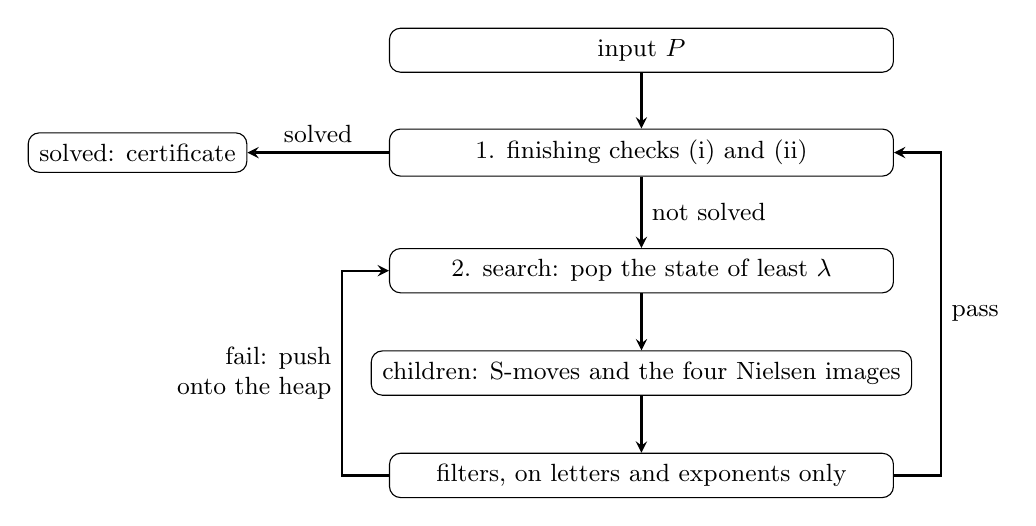
\begin{tikzpicture}[x=1cm,y=1cm,font=\small,
  box/.style={draw,rounded corners,align=center,inner sep=4pt,minimum width=6.4cm},
  arr/.style={->,>=stealth,thick}]
  \node[box] (in) at (0,0) {input $P$};
  \node[box] (fin) at (0,-1.3) {1. finishing checks (i) and (ii)};
  \node[draw,rounded corners,inner sep=4pt] (out) at (-6.4,-1.3) {solved: certificate};
  \node[box] (pop) at (0,-2.8) {2. search: pop the state of least $\lambda$};
  \node[box] (kids) at (0,-4.1) {children: S-moves and the four Nielsen images};
  \node[box] (filt) at (0,-5.4) {filters, on letters and exponents only};
  \draw[arr] (in) -- (fin);
  \draw[arr] (fin.west) -- node[above]{solved} (out);
  \draw[arr] (fin) -- node[right]{not solved} (pop);
  \draw[arr] (pop) -- (kids);
  \draw[arr] (kids) -- (filt);
  \draw[arr] (filt.west) -- ++(-0.6,0) |- node[pos=0.25,left,align=right]{fail: push\\onto the heap} (pop.west);
  \draw[arr] (filt.east) -- ++(0.6,0) |- node[pos=0.25,right,align=left]{pass} (fin.east);
\end{tikzpicture}
\caption{The hybrid solver. A child that passes the filters goes to the finishing checks, which then finish it; the
other children are pushed onto the heap.}
\label{fig:hybrid}
\end{figure}

\newpage
\subsection{Benchmarks}\label{sec:benchmarks}

% ---------BENCHMARKS---------------

\paragraph{Benchmarks.} Every benchmark below is a list of balanced presentations of the trivial
group, all of rank $2$. An \emph{expansion} is one removal of a state from the search heap. For a
presentation $P$, $g(P)$ is the number of expansions GS-SUB \cite{FTS26}, that is, LENGTH
(Definition~\ref{def:length}), needs to solve $P$, and
$g_S(P)$ is the number of expansions our greedy search with the $\SMK$ priority (Definition~\ref{def:smk}) needs. Every method is charged in the same units, one per expansion (Section~\ref{sec:units}).

\begin{definition}[MS640]
The Miller--Schupp benchmark of \cite{SMM24} is a list of $1{,}190$ presentations $\MS(n,w)$. \textbf{MS640}
\cite{FTS26} is the sublist of the $640$ presentations with $g(P)\le10^6$. Under $\Aut(\F_2)$, MS640, in particular, has $113$ orbits.
\end{definition}

\begin{definition}[bench60]\label{def:bench60}
\textbf{bench60} is a subset of $60$ presentations of MS640, comprising $6$ presentations from each of $10$ difficult class of
$g$ whose bounds increase geometrically by a factor of approximately $3.37$. Within each bin, the presentations are
chosen to span the range of path lengths and to minimise the number of pairs lying in a common $\Aut(\F_2)$-orbit. The
complete selection rule and position of the chosen presentations within MS640 are given in
Appendix~\ref{app:bench60}.
\end{definition}

\begin{definition}[AC19\_autmin]\label{def:ac19}
\textbf{AC19\_autmin} is the extended AC19 data set of \cite{FTS26} ($156{,}762$ balanced
presentations of the trivial group), reduced to one presentation per $\Aut(\F_2)$-orbit.
It has $72{,}779$ rows.
\end{definition}

A presentation of AC19 is AC-trivial if and only if its automorphic form is, so AC19\_autmin
carries the same AC-triviality questions as AC19. However, an automorphism of a presentation can be much harder or easier to search than the original presentation \cite{FTS26}.

\begin{definition}[ladder100]\label{def:ladder}\label{def:levels}
\textbf{ladder100} is a benchmark of $100$ AC-trivial presentations, taken from AC19\_autmin and MS640 and arranged
in $10$ levels of $10$ presentations each, in increasing order of difficulty for greedy search
(Figure~\ref{fig:ladder}). The selection rule within each level, the verification of AC-triviality and the statistics of each level are given in
Appendix~\ref{app:ladder}.
\end{definition}

The purpose of ladder100 is to extend the range of difficulty beyond that of MS640, up to presentations that are
AC-trivial but are not solved by greedy substitution search within $10^7$ expansions, and thereby to support the
development of algorithms for presentations closer to the second hump \cite{FTS26}.

\begin{figure}[ht]
\centering
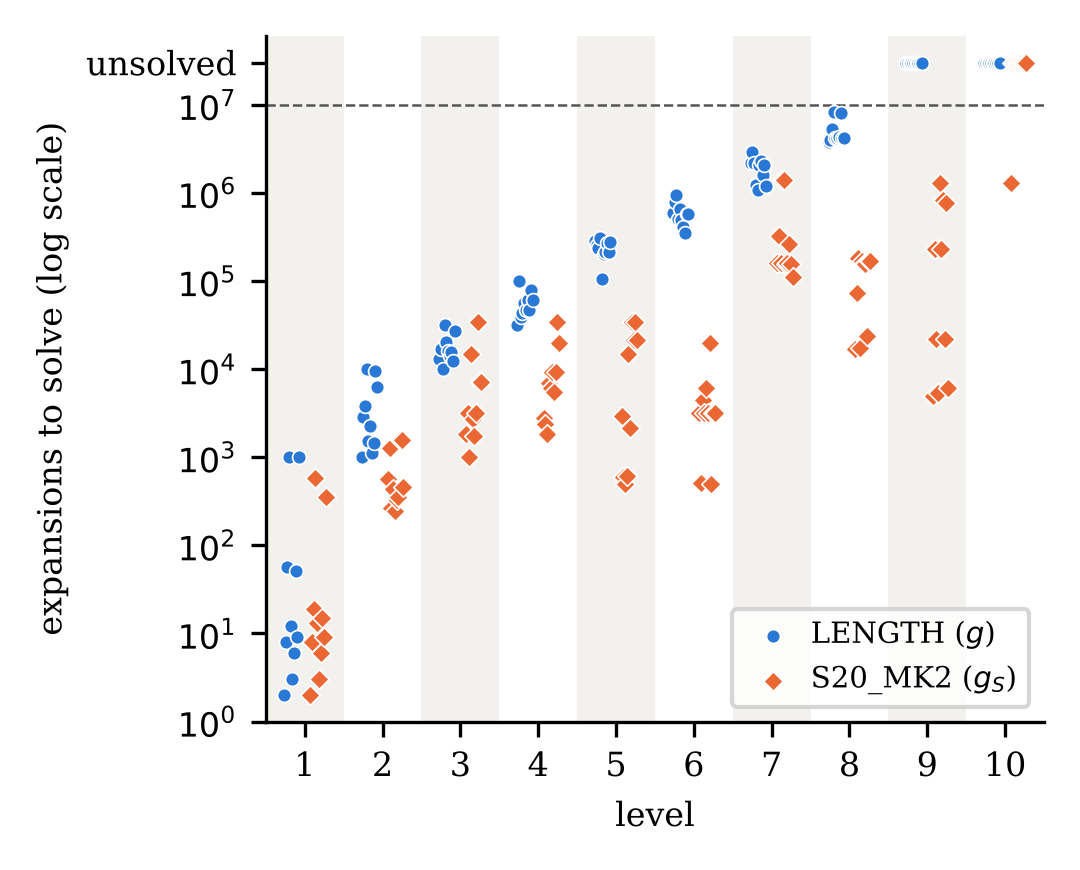
\includegraphics[width=0.6\textwidth]{figures/ladder100_levels.png}
\caption{The $100$ presentations of ladder100 by level: the number of expansions that LENGTH ($g$, circles) and
$\SMK$ ($g_S$, diamonds) require to solve each presentation. Searches that fail within $10^7$ expansions are placed
in the top row.}
\label{fig:ladder}
\end{figure}

\subsection{Units}\label{sec:units}

\paragraph{Units.} Every budget is counted in \emph{units}, and every method is charged one unit per
\emph{expansion}: the first state is removed from the heap, its children are generated, those already discovered are
discarded, and the remainder are pushed onto the heap according to the priority. For the hybrid
(Definition~\ref{def:hybrid}), each S-move applied by a finishing check is also charged one unit. A budget applies to
each presentation separately, a failed search is charged the full budget, and path lengths are counted in S-moves (for
the hybrid, S-moves together with Nielsen images).

An expansion does not require the same time in every method. Measured on a common set of states
(Appendix~\ref{app:time}), one expansion of $\SMK$ takes on average approximately $1.2$ times as long as one expansion
of LENGTH, one expansion of the hybrid approximately $2.1$ times as long, and the construction of the
change-of-variables images of a state approximately $3.6$ times as long. In this paper every method is nevertheless
charged one unit per expansion, so that equal budgets in units are comparable up to these factors.

\subsection{Results}\label{sec:ac_results}

\paragraph{Scores.} We compare the three methods at equal budgets in units: the number of
presentations each solves on the three benchmarks.
 
\begin{center}
\small
\begin{tabular}{llrrrrr}
\toprule
& & \multicolumn{5}{c}{budget (units)}\\
\cmidrule(lr){3-7}
benchmark & method & $10^3$ & $10^4$ & $10^5$ & $10^6$ & $10^7$\\
\midrule
MS640 & LENGTH & $554$ & $606$ & $634$ & $640$ & $640$\\
(of $640$) & $\SMK$ & $574$ & $626$ & $640$ & $640$ & $640$\\
& hybrid & $640$ & $640$ & $640$ & $640$ & $640$\\
\midrule
bench60 & LENGTH & $29$ & $40$ & $54$ & $60$ & $60$\\
(of $60$) & $\SMK$ & $37$ & $52$ & $60$ & $60$ & $60$\\
& hybrid & $60$ & $60$ & $60$ & $60$ & $60$\\
\midrule
ladder100 & LENGTH & $11$ & $20$ & $40$ & $60$ & $80$\\
(of $100$) & $\SMK$ & $23$ & $53$ & $69$ & $87$ & $91$\\
& hybrid & $99$ & $100$ & $100$ & $100$ & $100$\\
\bottomrule
\end{tabular}
 
\end{center}
 
$\SMK$ solves all of MS640 and bench60 by $10^5$ units, LENGTH only by $10^6$. On ladder100 neither finishes by
$10^7$: $9$ rows are unsolved by both. The hybrid solves all of MS640 and bench60 at $10^3$ units and all of
ladder100 at $10^4$; its hardest row, \texttt{ac19\_70845}, takes $2{,}267$ units.
 
\paragraph{Units and path lengths.} For every solve we also record the units it took and the length of its path:
S-moves. For the hybrid, each S-move and each Nielsen map counts as one unit; its path length is then rewritten as a sequence of AC moves on the original presentation and verified there.
 
\begin{center}
\small
\begin{tabular}{llrrrrrr}
\toprule
& & \multicolumn{3}{c}{units to solve} & \multicolumn{3}{c}{path length}\\
\cmidrule(lr){3-5}\cmidrule(lr){6-8}
benchmark & method & mean & median & max & mean & median & max\\
\midrule
MS640 & LENGTH & $4{,}963$ & $11$ & $574{,}959$ & $36.8$ & $9$ & $708$\\
 & $\SMK$ & $995$ & $11$ & $34{,}438$ & $42.9$ & $9$ & $787$\\
 & hybrid & $23$ & $11$ & $322$ & $21.2$ & $10$ & $262$\\
\midrule
bench60 & LENGTH & $45{,}244$ & $1{,}311$ & $574{,}959$ & $142.6$ & $47$ & $708$\\
 & $\SMK$ & $4{,}685$ & $359$ & $34{,}438$ & $154.3$ & $42$ & $787$\\
 & hybrid & $67$ & $28$ & $322$ & $59.9$ & $22$ & $262$\\
\midrule
ladder100 & LENGTH & $975{,}165$ & $101{,}771$ & $8{,}204{,}360$ & $130.8$ & $69$ & $706$\\
 & $\SMK$ & $114{,}830$ & $6{,}073$ & $1{,}383{,}279$ & $133.9$ & $69$ & $787$\\
 & hybrid & $127$ & $53$ & $2{,}267$ & $49.7$ & $30$ & $262$\\
\bottomrule
\end{tabular}
 
\smallskip
\footnotesize Over the rows each method solves (on ladder100: $80$, $91$ and $100$).
\end{center}
 
 
On easy rows the hybrid spends about as many units as the greedy searches (median $11$ against $11$ on MS640); on
hard rows it needs far fewer, at most $2{,}267$ against $8.2$ million for LENGTH.
Its paths are shorter on hard rows too: on the $80$ ladder100 rows that all three solve, $53.8$ steps on average
against $130.8$ for LENGTH and $142.4$ for $\SMK$. $\SMK$ paths are about as long as LENGTH's.

\clearpage
\section{Stable AC algorithms}\label{sec:stable}

\begin{definition}[Stable AC moves]\label{def:stableac}
The \emph{AC moves} on a presentation $P=\pres{X}{R}$ with $X=\{x_1,\dots,x_n\}$ and $R=\{r_1,\dots,r_n\}$ are (AC1) $r_i\mapsto r_ir_j$ for $i\neq j$, (AC2) $r_i\mapsto
r_i^{-1}$ and (AC3) $r_i\mapsto gr_ig^{-1}$ for $g\in X^{\pm1}$. The \emph{trivial presentation} is $\pres{X}{X}$.
The \emph{stable AC moves} add two more, for a generator $z\notin X$:
\begin{align*}
&(\mathrm{AC4})\quad \pres{X}{R}\ \longmapsto\ \pres{X,z}{R,\,z},\\
&(\mathrm{AC5})\quad \pres{X,z}{R,\,z}\ \longmapsto\ \pres{X}{R},\qquad\text{if $z$ does not occur in $R$}.
\end{align*}
$P$ is \emph{stably AC-trivial} if AC1--AC5 take $P$ to the trivial presentation.
\end{definition}

\begin{definition}[Stabilized start]\label{def:stab}
For $P=\pres{x,y}{r_1,r_2}$ and words $w_1,\dots,w_k$ in $x,y$, the \emph{stabilized start} is
\[
P_w=\pres{x,y,z_1,\dots,z_k}{r_1,\ r_2,\ z_1^{-1}w_1,\ \dots,\ z_k^{-1}w_k},
\]
of rank $2+k$. For example, $w=xy$ gives $\pres{x,y,z}{r_1,r_2,z^{-1}xy}$: the new generator $z$ stands for $xy$.
\end{definition}

If $P$ presents the trivial group, then $P$ and $P_w$ are related by stable AC moves \cite[Lemma~11]{SMM24}. So an
AC path from $P_w$ to the trivial presentation shows that $P$ is stably AC-trivial. 
presents the trivial group.

\begin{definition}[Naive stable search]\label{def:naive}
LENGTH (Definition~\ref{def:length}) run on $P_w$: S-moves between any two of the $2+k$ relators, with the same
priority $\lambda$. For $k=0$ it is LENGTH on $P$, the rank-$2$ baseline.
\end{definition}

\paragraph{Setup.} All searches are on the $640$ presentations of MS640, with a budget of $10^3$ units per search
unless stated otherwise. A \emph{start} is a choice of the words $w_1,\dots,w_k$ of Definition~\ref{def:stab}, and one search is one run of the naive stable search from one start on one presentation.

The rank-$3$ starts ($k=1$) are the freely reduced words $w$ of length $1$ to $10$, taken up to inversion, that is
$59{,}048$ words; the words of length $1$ to $7$ are also run at a budget of $10^4$ units. The construction of these
words, and the derivation of their number, are given in Appendix~\ref{app:stable}.

For each word length $n$, three measures are reported, each as a number of presentations out of $640$; they are the
three curves of Figure~\ref{fig:stable_words}.
\begin{itemize}
  \item \emph{Random word}: every word of length exactly $n$ is run on every presentation, and the total number of
  solves is divided by the number of words. It is the number of presentations that a word of length $n$, chosen at
  random, solves on average. For $n=1$, the $2$ words solve $769$ of the $2\times640=1{,}280$ searches, that is
  $384.5$ presentations per word; for $n=10$, the $39{,}366$ words solve $16{,}550{,}697$ of the $39{,}366\times640$
  searches, that is $420.4$ presentations per word.
  \item \emph{Best fixed word}: the largest number of presentations solved by a single word of length at most $n$,
  the same word being used on every presentation. The word is chosen after the searches, with hindsight.
  \item \emph{Some word}: the number of presentations solved by at least one word of length at most $n$, each
  presentation being allowed its own word. It requires the right word for each presentation in advance, so it is an
  upper bound on what any choice of word can achieve, and not itself a method.
\end{itemize}
Each measure is compared with rank $2$, that is, LENGTH on $P$, which solves $554$ presentations at $10^3$ units and
$606$ at $10^4$ units.

\begin{figure}[ht]
\centering
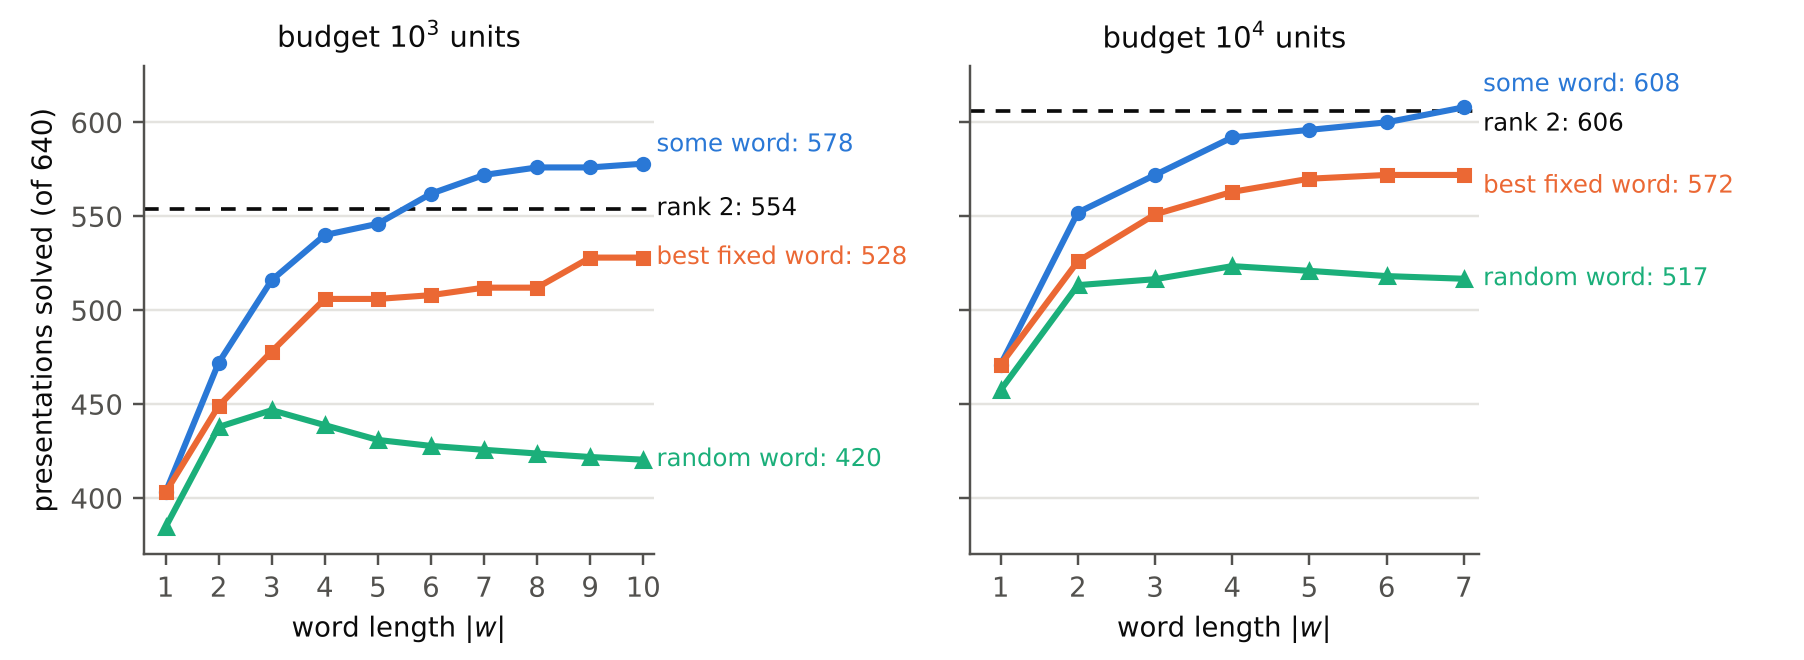
\includegraphics[width=\textwidth]{figures/stable_rank3_words.png}
\caption{Rank 3 against rank 2 on MS640. Some word and the best fixed word use the words of length at most $|w|$;
random word is $640$ times the share solved by the words of length exactly $|w|$. Dashed: rank 2. Rank 3 beats rank 2 only with the right word (Figure~\ref{fig:stable_words},
Table~\ref{tab:stable_words}). A random word solves at most $446.8$ presentations on average, against $554$ for
rank 2, and the best fixed word, \texttt{yXYYYxyyy}, solves $528$. }
\label{fig:stable_words}
\end{figure}

\begin{table}[ht]
\centering
\small
\textbf{Naive stable search: rank 3 against rank 2 on MS640}\par\smallskip
\begin{tabular}{rrrrrrr}
\toprule
& & \multicolumn{2}{c}{words of length $|w|$} & \multicolumn{3}{c}{some word of length $\le|w|$}\\
\cmidrule(lr){3-4}\cmidrule(lr){5-7}
$|w|$ & words & random word & faster than rank 2 & solves & gained & lost\\
\midrule
1 & $2$ & $384.5$ & $0.0\%$ & $403$ & $0$ & $151$\\
2 & $6$ & $437.8$ & $1.1\%$ & $472$ & $0$ & $82$\\
3 & $18$ & $446.8$ & $0.6\%$ & $516$ & $0$ & $38$\\
4 & $54$ & $438.8$ & $1.1\%$ & $540$ & $4$ & $18$\\
5 & $162$ & $430.9$ & $0.9\%$ & $546$ & $8$ & $16$\\
6 & $486$ & $427.8$ & $0.7\%$ & $562$ & $16$ & $8$\\
7 & $1{,}458$ & $425.7$ & $0.6\%$ & $572$ & $20$ & $2$\\
8 & $4{,}374$ & $423.7$ & $0.6\%$ & $576$ & $22$ & $0$\\
9 & $13{,}122$ & $421.8$ & $0.5\%$ & $576$ & $22$ & $0$\\
10 & $39{,}366$ & $420.4$ & $0.5\%$ & $578$ & $24$ & $0$\\
\midrule
rank 2 & & $554$ & & $554$ & &\\
\bottomrule
\end{tabular}
\caption{Rank 3 at budget $10^3$. Faster: the share of the $640\times$words searches solved in fewer units than rank 2. Some word: the presentations solved by at least one word of length at most $|w|$. Gained: solved by some word, not by rank 2; lost: solved by
rank 2, by no word.}
\label{tab:stable_words}
\end{table}

\clearpage

\subsection{Change of variables}\label{sec:cov}

The naive stable search keeps $z$ and searches in rank $3$. A change of variables uses $z$ once, to remove $x$ or $y$,
and then searches in rank $2$ again.

\begin{definition}[Change of variables]\label{def:cov}
Let $P=\pres{x,y}{r_1,r_2}$ and let $w$ be a word in $x,y$ of length at least $2$.
\begin{enumerate}
  \item \emph{Stabilize}: $P_w=\pres{x,y,z}{r_1,\ r_2,\ z^{-1}w}$ (Definition~\ref{def:stab}).
  \item \emph{Substitute}: replace non-overlapping occurrences of $w^{\pm1}$ in $r_1,r_2$ by $z^{\pm1}$ and freely
  reduce. Call the results $r_1',r_2'$.
  \item \emph{Eliminate}: choose one of $r_1',r_2',z^{-1}w$ in which a generator $g\in\{x,y\}$ occurs exactly once.
  Write it cyclically as $g^{\epsilon}s$, with $g$ not in $s$, so that $g=s^{-\epsilon}$ in the group. Substitute
  $s^{-\epsilon}$ for $g$ in the other two relators and delete the chosen one.
\end{enumerate}
The result is a presentation $P'$ on the two generators $\{x,y,z\}\setminus\{g\}$, the \emph{image} of $P$. We rename
them $x,y$ and search $P'$ with LENGTH.
\end{definition}

An example is given in Appendix~\ref{app:cov}.

The searches of this section use the following family of images.

\begin{definition}[CoV images of a state]\label{def:covimages}
For a state $Q=\pres{x,y}{r_1,r_2}$, the \emph{CoV images} of $Q$ are the images (Definition~\ref{def:cov}) obtained
from every word $w$ that is a cyclic subword of $r_1$ or of $r_2$ with $2\le|w|\le|r_i|-1$, by substituting every
non-empty set of non-overlapping occurrences of $w^{\pm1}$ and eliminating every generator $g$ through every relator
in which $g$ occurs once. Images equal up to relator order, rotation, inversion and the $8$ signed permutations of
$x,y$ are identified, and an image equal to $Q$ is discarded. No length bound is applied.
\end{definition}

A CoV image is an automorphic image of $Q$ when the relator used for the elimination contains $z$ exactly once; a
solve whose CoV moves are all of this kind is transported to an AC path of $P$. Otherwise the solve is a stable
certificate \cite[Lemma~11]{SMM24}.

\paragraph{One-shot CoV.}

\begin{definition}[One-shot CoV]\label{def:oneshot}
The \emph{one-shot CoV} search runs LENGTH on a single CoV image of $P$ (Definition~\ref{def:covimages}) in place of
$P$.
\end{definition}

On MS640 the presentations have $5$ to $10{,}740$ CoV images (median $36$), $114{,}042$ in all, and every image was
searched. As for rank $3$, Table~\ref{tab:cov_all} reports two measures, each as a number of presentations out of
$640$, and compares them with LENGTH on $P$.
\begin{itemize}
  \item \emph{Random image}: the share of the images of $P$ that are solved, summed over the $640$ presentations. It is
  the number of presentations that an image chosen at random solves on average.
  \item \emph{Best image}: the number of presentations solved by at least one of their images. Like some word, it
  requires the right image for each presentation in advance, so it is an upper bound and not a method; the last
  column gives the mean number of units needed to search every image.
\end{itemize}

\begin{table}[ht]
\centering
\small
\textbf{One-shot CoV against LENGTH on MS640}\par\smallskip
\begin{tabular}{rrrrrr}
\toprule
budget & LENGTH & random & best & & units to search\\
per search & on $P$ & image & image & gained & every image\\
\midrule
$10$ & $317$ & $271.7$ & $416$ & $99$ & $1{,}408$\\
$10^2$ & $455$ & $430.8$ & $555$ & $100$ & $5{,}328$\\
$10^3$ & $554$ & $527.0$ & $604$ & $50$ & $28{,}456$\\
$10^4$ & $606$ & $581.4$ & $626$ & $20$ & $164{,}759$\\
$10^5$ & $634$ & $613.2$ & $640$ & $6$ & $657{,}198$\\
\bottomrule
\end{tabular}
\caption{Gained: solved by the best image, not by LENGTH on $P$; no presentation is lost. Units to search every image:
the mean over presentations, a failed search counted at the full budget. Images are searched with the length bound
$\max(24,\ \text{longest relator}+16)$, $P$ with $24$.}
\label{tab:cov_all}
\end{table}

The best image passes LENGTH at every budget, but the margin falls from $100$ to $6$, and finding the image costs more
than the margin. A random image solves fewer presentations than LENGTH on $P$ at every budget.

\FloatBarrier
\paragraph{Searches with change-of-variables moves.} The searches below use the change of variables as a move inside
a search rather than once at the start.

\begin{definition}[CoV-gate search]\label{def:covgate}
The \emph{CoV-gate search} of \cite{Zan} is a greedy search with priority $\lambda$, ties broken by depth and then by
order of insertion, and no length bound. An expansion of a state $Q$ generates its S-move children; if no S-move
child is shorter than $Q$ (the gate \emph{opens}), it also generates the CoV images of $Q$. In \cite{Zan} the CoV
move substitutes a single occurrence of a cyclic window, so that every CoV move is an automorphism; here it is
replaced by the CoV images of Definition~\ref{def:covimages}. One unit is charged per expansion and one more per
opening of the gate.
\end{definition}

\begin{definition}[Dual and triple searches]\label{def:dualtriple}
The searches of \cite{Ste} keep several heaps, each ordered by $\lambda$ with ties broken towards the deepest state.
Every new state is pushed onto the \emph{S-heap}, and a state removed from the S-heap is expanded by S-moves and then
pushed onto the other heaps. Removing a state from a CoV heap generates its CoV children, which are pushed onto the
S-heap. One unit is charged per removal from any heap, and the input is expanded once by the CoV heaps without charge.
\begin{itemize}
  \item \emph{Dual, single CoV}: one CoV heap, whose children are the CoV images. The CoV heap is used when its first
  state is at least $3$ shorter than the first state of the S-heap, and the S-heap otherwise.
  \item \emph{Dual, auto CoV}: as the dual, single CoV, with the children of the CoV heap being the $24$ images under
  $x\mapsto xy^{k}$ and $y\mapsto yx^{k}$, $1\le|k|\le6$, together with the CoV images.
  \item \emph{Triple}: an S-heap, an auto heap with the $24$ images above, and a CoV heap with the CoV images. Each
  step uses the heap of least $\lambda+t$, with $t=0$ for the S-heap and $t=2$ for the other two, ties going to the
  S-heap, then the auto heap.
\end{itemize}
In \cite{Ste} the CoV step of the dual is a single substitution, and that of the triple substitutes at least two
occurrences; here both are replaced by the CoV images of Definition~\ref{def:covimages}.
\end{definition}

\paragraph{Scores.} Table~\ref{tab:cov_search_solved} gives the number of presentations each search solves at equal
budgets in units, and Table~\ref{tab:cov_search_paths} the units and path lengths of the solves. A path length counts
each S-move and each CoV move as one step. Every solve was replayed move by move.

\begin{table}[ht]
\centering
\small
\begin{tabular}{llrrrrr}
\toprule
& & \multicolumn{5}{c}{budget (units)}\\
\cmidrule(lr){3-7}
benchmark & method & $10^3$ & $10^4$ & $10^5$ & $10^6$ & $10^7$\\
\midrule
MS640 & LENGTH & $554$ & $606$ & $634$ & $640$ & $640$\\
(of $640$) & $\SMK$ & $574$ & $626$ & \underline{$640$} & $640$ & $640$\\
 & hybrid & \underline{$640$} & \underline{$640$} & \underline{$640$} & $640$ & $640$\\
 & CoV gate & $596$ & $612$ & $626$ & $640$ & $640$\\
 & dual, single CoV & $612$ & $634$ & \underline{$640$} & $640$ & $640$\\
 & dual, auto CoV & $612$ & $627$ & \underline{$640$} & $640$ & $640$\\
 & triple & $612$ & $637$ & \underline{$640$} & $640$ & $640$\\
\midrule
bench60 & LENGTH & $29$ & $40$ & $54$ & $60$ & $60$\\
(of $60$) & $\SMK$ & $37$ & $52$ & \underline{$60$} & $60$ & $60$\\
 & hybrid & \underline{$60$} & \underline{$60$} & \underline{$60$} & $60$ & $60$\\
 & CoV gate & $45$ & $49$ & $52$ & $60$ & $60$\\
 & dual, single CoV & $49$ & $57$ & \underline{$60$} & $60$ & $60$\\
 & dual, auto CoV & $49$ & $53$ & \underline{$60$} & $60$ & $60$\\
 & triple & $49$ & $58$ & \underline{$60$} & $60$ & $60$\\
\midrule
ladder100 & LENGTH & $11$ & $20$ & $40$ & $60$ & $80$\\
(of $100$) & $\SMK$ & $23$ & $53$ & $69$ & $87$ & $91$\\
 & hybrid & \underline{$99$} & \underline{$100$} & \underline{$100$} & \underline{$100$} & \underline{$100$}\\
 & CoV gate & $73$ & $89$ & $93$ & \underline{$100$} & \underline{$100$}\\
 & dual, single CoV & $73$ & $98$ & \underline{$100$} & \underline{$100$} & \underline{$100$}\\
 & dual, auto CoV & $72$ & $94$ & \underline{$100$} & \underline{$100$} & \underline{$100$}\\
 & triple & $73$ & $97$ & \underline{$100$} & \underline{$100$} & \underline{$100$}\\
\bottomrule
\end{tabular}
\caption{Presentations solved by the searches with CoV images, with LENGTH, $\SMK$ and the hybrid
(Section~\ref{sec:ac_results}) for comparison. The CoV-gate search has been run to $10^6$ units, by which it solves
every presentation. In each benchmark, the largest number in each column is underlined, unless all methods tie.}
\label{tab:cov_search_solved}
\end{table}

\begin{figure}[ht]
\centering
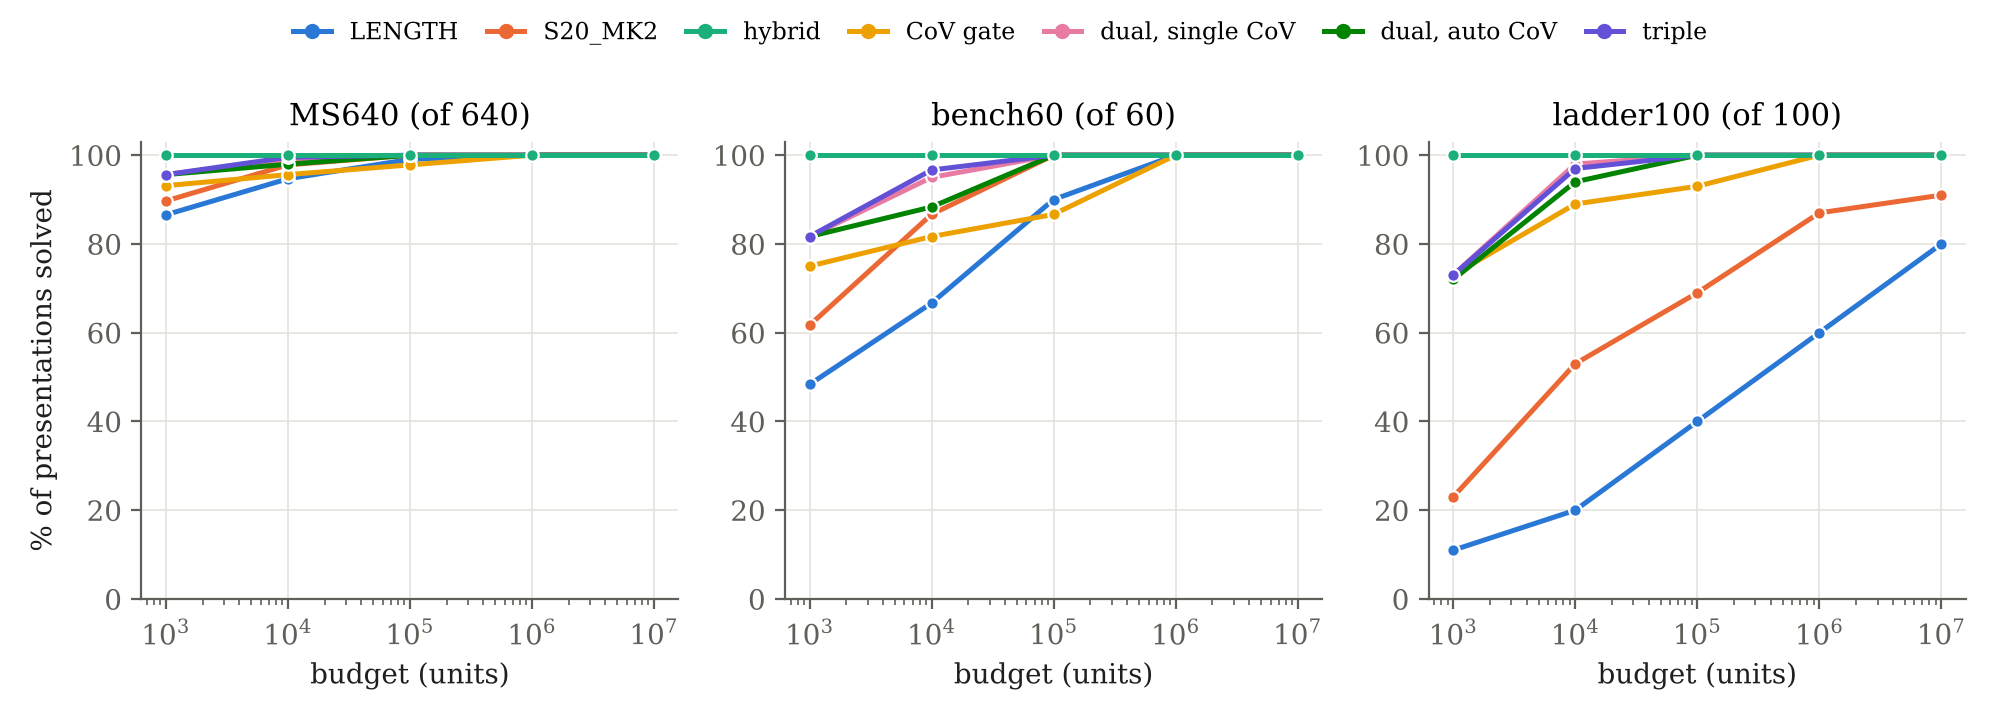
\includegraphics[width=\textwidth]{figures/scores_budget.png}
\caption{The numbers of Table~\ref{tab:cov_search_solved} as a percentage of each benchmark: presentations solved
against the budget in units, counted exactly at four budgets per decade. The dual, auto CoV search, which never solves more than the dual, single CoV search, is
omitted.}
\label{fig:scores_budget}
\end{figure}

\begin{table}[ht]
\centering
\small
\begin{tabular}{llrrrrrr}
\toprule
& & \multicolumn{3}{c}{units to solve} & \multicolumn{3}{c}{path length}\\
\cmidrule(lr){3-5}\cmidrule(lr){6-8}
benchmark & method & mean & median & max & mean & median & max\\
\midrule
MS640 & CoV gate & $4{,}104$ & $10$ & $149{,}552$ & \underline{$20.5$} & \underline{$8$} & \underline{$375$}\\
& dual, single CoV & \underline{$305$} & $9$ & $19{,}544$ & $41.2$ & $9$ & $963$\\
& dual, auto CoV & $579$ & \underline{$8$} & $31{,}332$ & $40.2$ & \underline{$8$} & $907$\\
& triple & $312$ & \underline{$8$} & \underline{$18{,}528$} & $39.2$ & \underline{$8$} & $842$\\
\midrule
bench60 & CoV gate & $21{,}827$ & \underline{$27.5$} & $149{,}552$ & \underline{$70.2$} & \underline{$16.5$} & \underline{$375$}\\
& dual, single CoV & \underline{$1{,}576$} & $106$ & $19{,}544$ & $162.5$ & $25.5$ & $963$\\
& dual, auto CoV & $3{,}055$ & $120$ & $31{,}016$ & $152.6$ & $25.5$ & $907$\\
& triple & $1{,}657$ & $114$ & \underline{$18{,}528$} & $145.8$ & $32.5$ & $842$\\
\midrule
ladder100 & CoV gate & $12{,}119$ & \underline{$96$} & $149{,}552$ & \underline{$50.4$} & \underline{$20$} & \underline{$375$}\\
& dual, single CoV & \underline{$1{,}146$} & $290$ & \underline{$10{,}372$} & $118.0$ & $46$ & $941$\\
& dual, auto CoV & $2{,}059$ & $426$ & $31{,}016$ & $116.3$ & $48$ & $907$\\
& triple & $1{,}444$ & $403$ & $18{,}528$ & $113.2$ & $52$ & $842$\\
\bottomrule
\end{tabular}
\caption{Units and path lengths over the presentations each search solves (all of them, at $10^6$ units for the
CoV-gate search). In each benchmark, the smallest number in each column is underlined.}
\label{tab:cov_search_paths}
\end{table}

\FloatBarrier
\subsection{Total relator length on a solution path}\label{sec:maxrel}

A search may lengthen the relators of a presentation before it shortens them. For every solved presentation we
record the largest total relator length over all states of its solution path, the starting presentation included,
each relator cyclically reduced. For LENGTH and $\SMK$ the states are those of the S-move path. For the hybrid we give
two measures: over the states of its search, that is, the presentations after each S-move and each Nielsen map, and
over the states of its AC path, in which each Nielsen map is rewritten as a sequence of AC moves on the original
presentation. For the searches with CoV moves the states are the CoV images on the path; the intermediate
presentations with three generators are not counted, and the paths are not rewritten as AC moves.

\begin{table}[ht]
\centering
\small
\begin{tabular}{llrrrr}
\toprule
& & & \multicolumn{3}{c}{largest total relator length on the path}\\
\cmidrule(lr){4-6}
benchmark & method & start & mean & median & max\\
\midrule
MS640 & LENGTH & $16.1$ & $16.9$ & $16$ & $31$\\
 & $\SMK$ & $16.1$ & $17.6$ & $16$ & $35$\\
 & hybrid, search states & $16.1$ & $25.5$ & $16$ & $255$\\
 & hybrid, AC path & $16.1$ & $55.1$ & $17$ & $1{,}014$\\
 & CoV gate & $16.1$ & $16.2$ & $15$ & $25$\\
 & dual, single CoV & $16.1$ & $16.2$ & $15$ & $25$\\
 & dual, auto CoV & $16.1$ & $16.2$ & $15$ & $25$\\
 & triple & $16.1$ & $16.2$ & $15$ & $25$\\
\midrule
bench60 & LENGTH & $19.3$ & $22.0$ & $22.5$ & $31$\\
 & $\SMK$ & $19.3$ & $23.8$ & $23$ & $35$\\
 & hybrid, search states & $19.3$ & $59.3$ & $21$ & $255$\\
 & hybrid, AC path & $19.3$ & $214.8$ & $70.5$ & $1{,}014$\\
 & CoV gate & $19.3$ & $19.3$ & $20.5$ & $25$\\
 & dual, single CoV & $19.3$ & $19.4$ & $20.5$ & $25$\\
 & dual, auto CoV & $19.3$ & $19.4$ & $20.5$ & $25$\\
 & triple & $19.3$ & $19.4$ & $20.5$ & $25$\\
\midrule
ladder100 & LENGTH & $19.8$ & $27.8$ & $28.5$ & $39$\\
 & $\SMK$ & $19.9$ & $30.3$ & $31$ & $43$\\
 & hybrid, search states & $19.8$ & $45.1$ & $21$ & $255$\\
 & hybrid, AC path & $19.8$ & $242.1$ & $146$ & $1{,}014$\\
 & CoV gate & $19.8$ & $20.4$ & $21$ & $25$\\
 & dual, single CoV & $19.8$ & $20.5$ & $21$ & $25$\\
 & dual, auto CoV & $19.8$ & $20.5$ & $21$ & $25$\\
 & triple & $19.8$ & $20.5$ & $21$ & $25$\\
\bottomrule
\end{tabular}
\caption{The largest total relator length on the solution path, over the presentations each method solves (on
ladder100: $80$ for LENGTH, $91$ for $\SMK$, all $100$ for the others). Start: the mean total relator length of the
starting presentations, over the same presentations.}
\label{tab:maxrel}
\end{table}

The greedy searches and the searches with CoV moves stay close to the starting length: on MS640 the mean rises from
$16.1$ to at most $17.6$, and no path of these searches has a total length above $43$; a path of a search with CoV
moves exceeds the total length of its starting presentation by at most $4$. The hybrid's search states rise further,
to a mean of $25.5$ on MS640 and $45.1$ on ladder100 and at most $255$, and its AC paths further still, to at most
$1{,}014$: a Nielsen map rewritten as AC moves lengthens the relators temporarily. Since the paths of the
searches with CoV moves are not rewritten as AC moves, their figures compare with the hybrid's search states, not with
its AC path.

Figure~\ref{fig:maxrel_summary} shows the mean and the largest values of Table~\ref{tab:maxrel}, and
Figure~\ref{fig:maxrel_example} follows the presentation on which the hybrid's AC path reaches a total length of $1{,}014$.

\begin{figure}[ht]
\centering
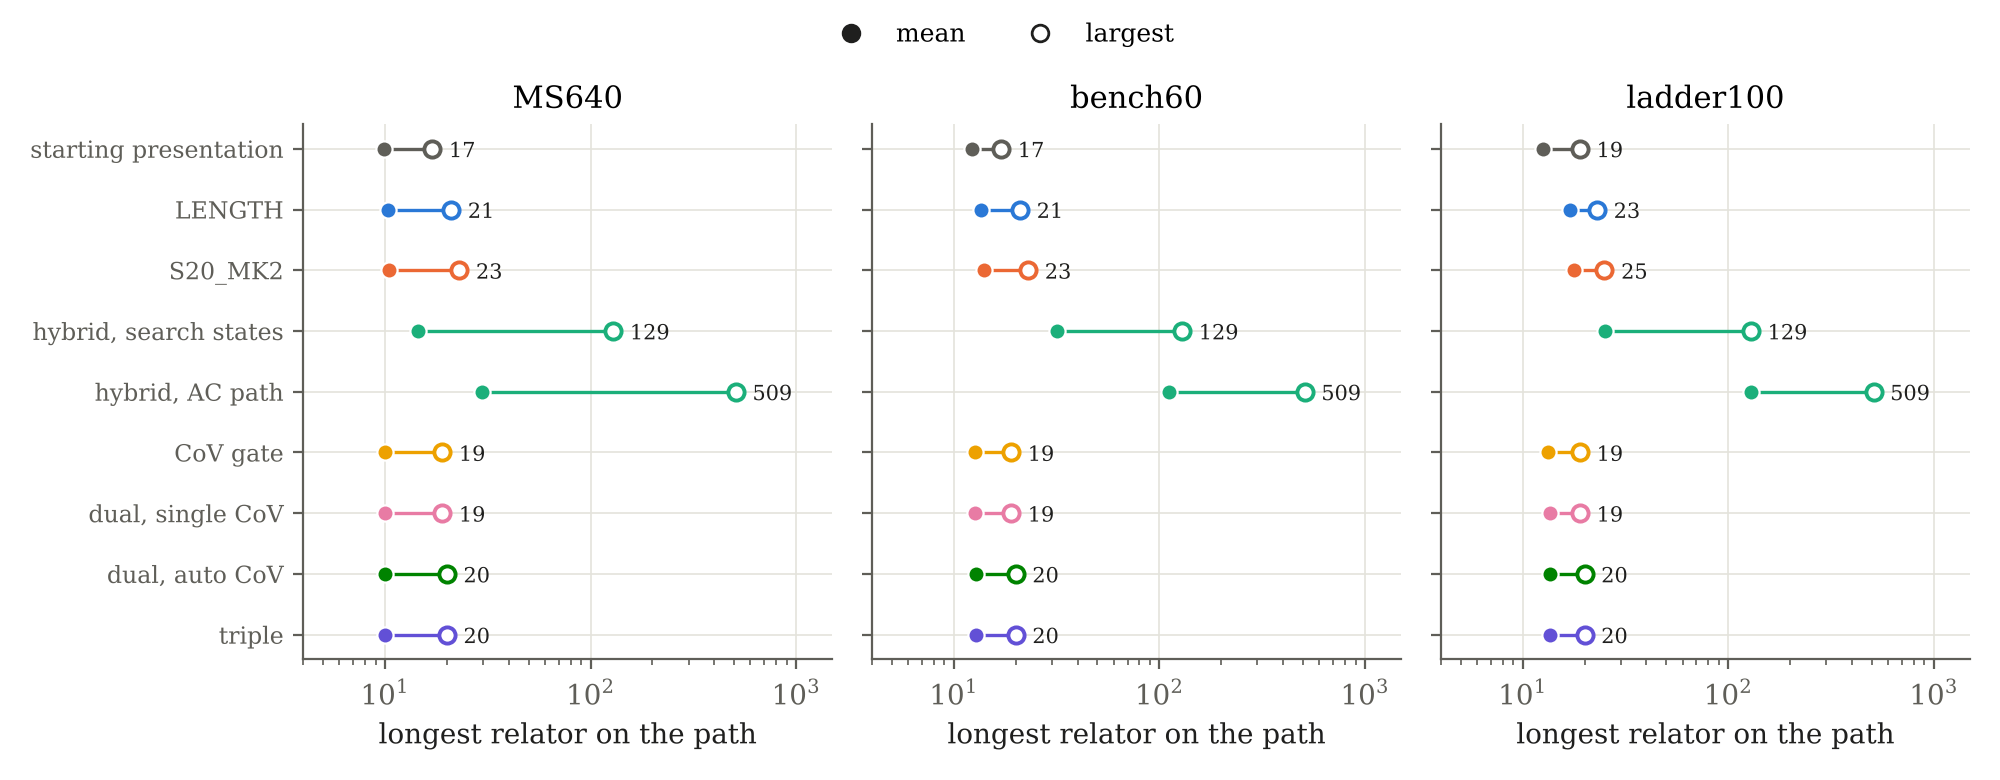
\includegraphics[width=\textwidth]{figures/maxrel_summary.png}
\caption{The largest total relator length on the solution path (Table~\ref{tab:maxrel}): the mean (filled) and the
largest value (open) over the presentations each method solves. Dashed: the mean total length of the starting
presentations. The horizontal axis is logarithmic.}
\label{fig:maxrel_summary}
\end{figure}

\begin{figure}[ht]
\centering
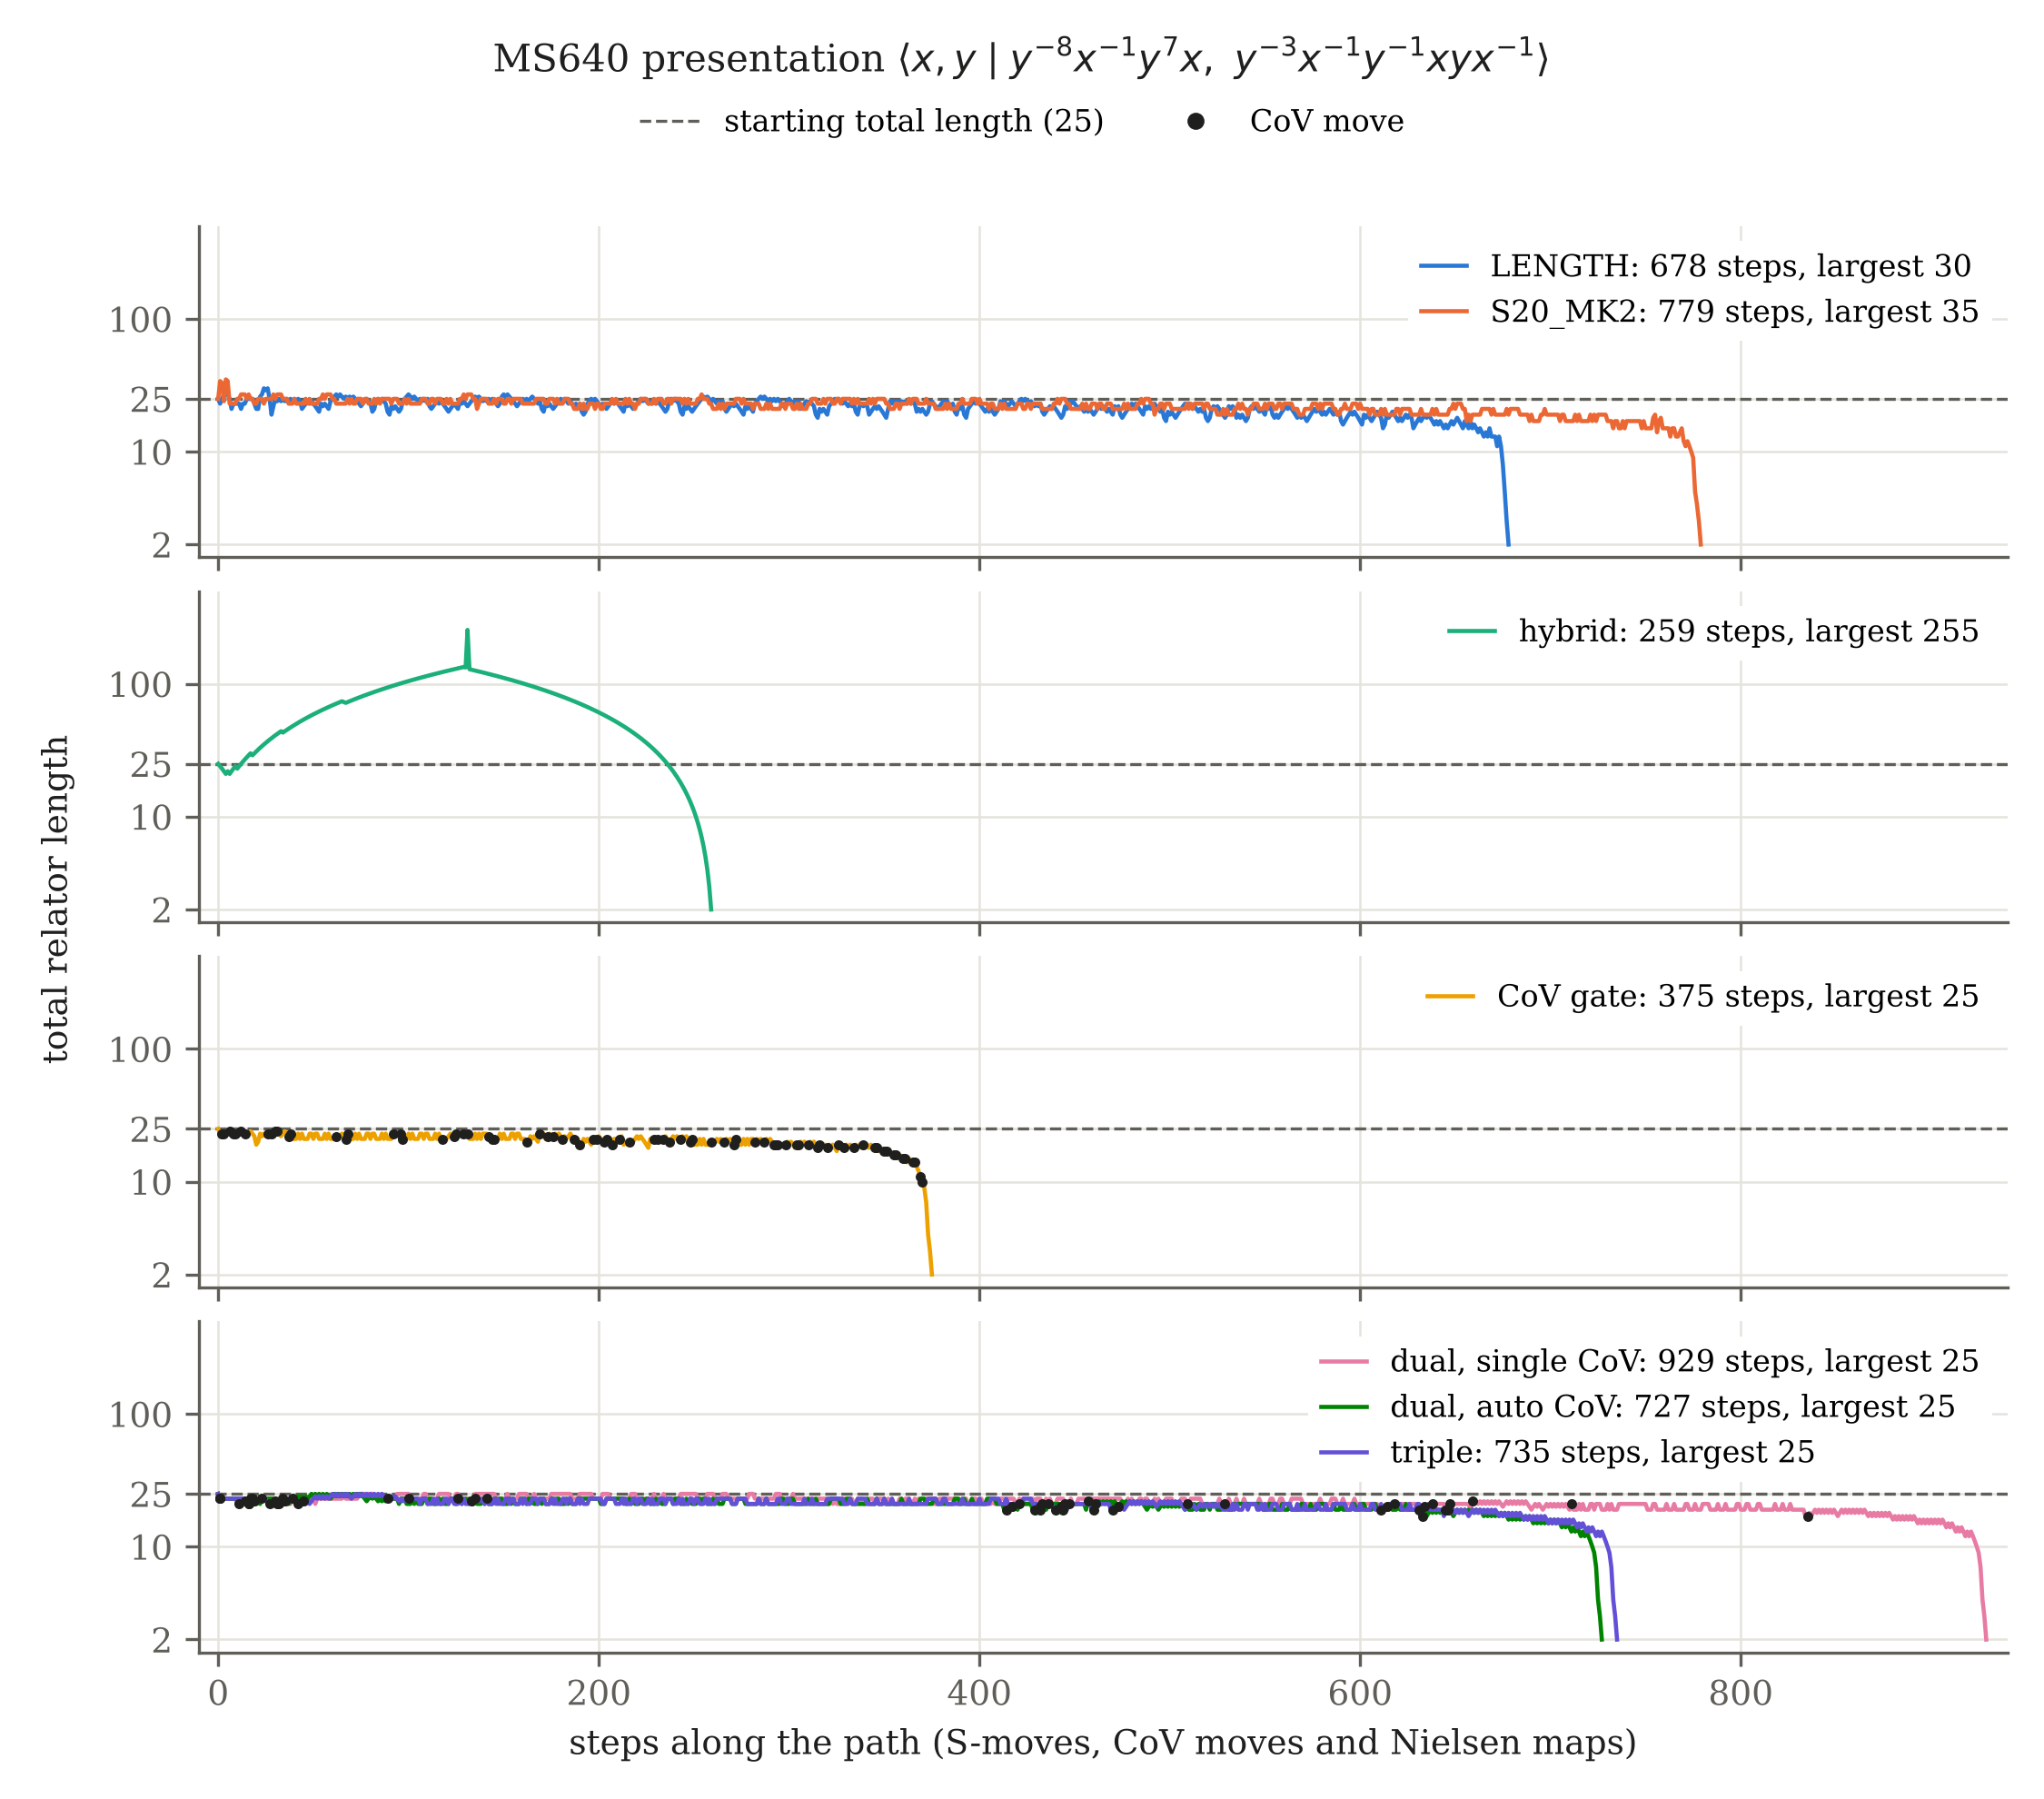
\includegraphics[width=\textwidth]{figures/maxrel_example.png}
\caption{The total relator length along the solution paths of the seven methods on the MS640 presentation
$\pres{x,y}{y^{-8}x^{-1}y^7x,\ y^{-3}x^{-1}y^{-1}xyx^{-1}}$, step by step, from top to bottom: LENGTH and $\SMK$; the
hybrid; the CoV-gate search; the dual and triple searches. A step is an S-move, a CoV move (black points) or a Nielsen map. Dashed: the total length of the presentation, $25$.
The vertical axis is logarithmic. Rewritten as AC moves on the original presentation ($2{,}783$ moves), the hybrid's
path reaches a total relator length of $1{,}014$, with a relator of length $509$.}
\label{fig:maxrel_example}
\end{figure}





\clearpage
\bibliographystyle{plain}
\bibliography{references}

\clearpage
% All appendices, in one file. avi.tex pulls it in with % All appendices, in one file. avi.tex pulls it in with % All appendices, in one file. avi.tex pulls it in with \input{appendix/appendix}; no preamble here.
% One big unnumbered section, "Appendix"; each part is a subsection lettered A, B, C, ...
% Add the next part as another \subsection{...}\label{app:...} below.
\section*{Appendix}\label{sec:appendix}
\addcontentsline{toc}{section}{Appendix}
\setcounter{subsection}{0}
\renewcommand{\thesubsection}{\Alph{subsection}}

\subsection{bench60}\label{app:bench60}

\begin{definition}[bench60, full rule]\label{def:bench60full}
Let $g_0=3$ and $g_{10}=574{,}959$ be the least and the largest value of $g$ on MS640 at budget $10^6$, and
let $\rho=(g_{10}/g_0)^{1/10}\approx3.37$. The \emph{difficulty class} $b\in\{0,\dots,9\}$ is the set of $P\in$ MS640 with
$g_0\rho^{b}\le g(P)<g_0\rho^{b+1}$ (class $9$ closed on the right). \textbf{bench60} takes $6$ presentations from every
difficulty class by the following rule.
\begin{enumerate}
  \item Over the whole subset, minimise the number of pairs of chosen presentations in the same $\Aut(\F_2)$-orbit.
  \item Subject to (1), sort the presentations of each difficulty class by path length, the number of S-moves in the solution GS-SUB finds; break ties by smaller $g$ first, then by line number in MS640.
  Take the $6$ presentations closest to $6$ evenly spaced positions of this sorted list, the first and the last
  position included.
  % This one needs more explaination
\end{enumerate}
\end{definition}

Figure~\ref{fig:bench60} shows where the $60$ rows lie in MS640.

\begin{center}
\begin{tabular}{rrrrr}
\toprule
class $b$ & range of $g$ & rows of MS640 & rows of bench60 & mean $g$ on bench60\\
\midrule
0 & $[3,\,11)$ & $317$ & $6$ & $6.3$\\
1 & $[11,\,35)$ & $89$ & $6$ & $17.7$\\
2 & $[35,\,116)$ & $63$ & $6$ & $74.3$\\
3 & $[116,\,390)$ & $60$ & $6$ & $261.7$\\
4 & $[390,\,1{,}314)$ & $31$ & $6$ & $691.2$\\
5 & $[1{,}314,\,4{,}433)$ & $26$ & $6$ & $1{,}746.8$\\
6 & $[4{,}433,\,14{,}959)$ & $28$ & $6$ & $9{,}869.2$\\
7 & $[14{,}959,\,50{,}482)$ & $14$ & $6$ & $19{,}596.3$\\
8 & $[50{,}482,\,170{,}367)$ & $6$ & $6$ & $66{,}530.7$\\
9 & $[170{,}367,\,574{,}959]$ & $6$ & $6$ & $353{,}647.7$\\
\midrule
all & & $640$ & $60$ & \\
\bottomrule
\end{tabular}
\end{center}

\begin{figure}[ht]
\centering
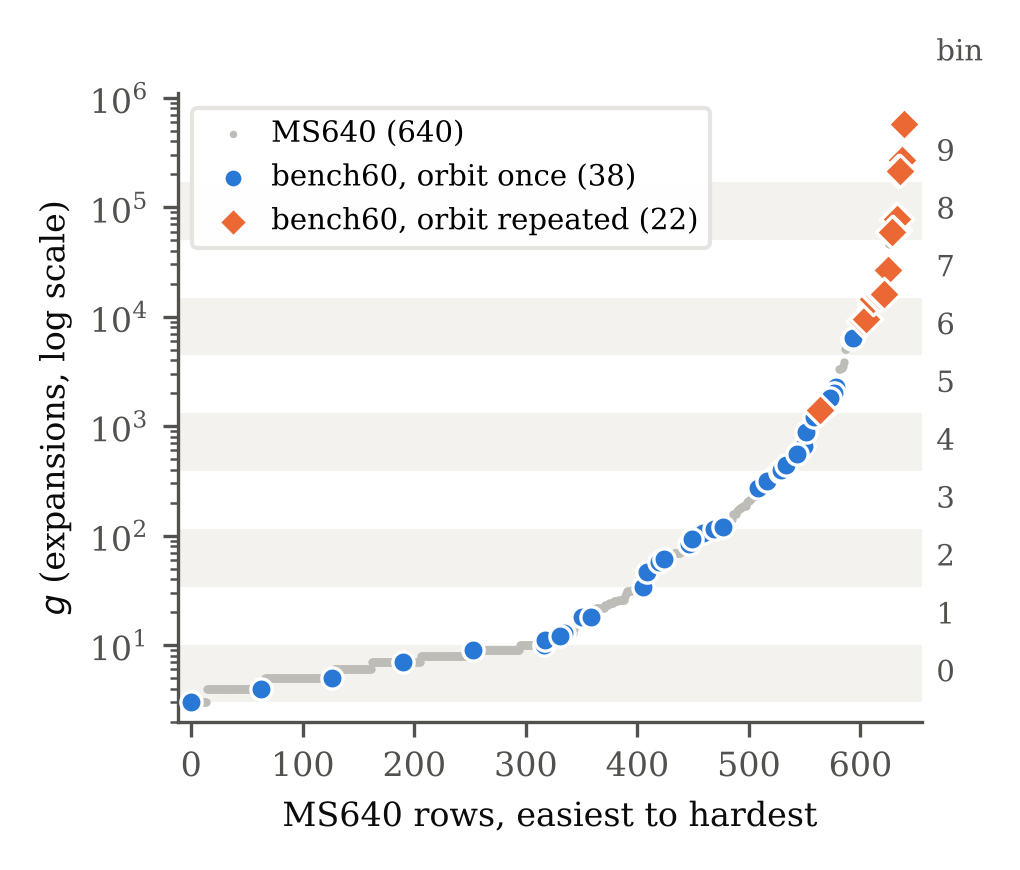
\includegraphics[width=0.49\textwidth]{figures/bench60_g.png}\hfill
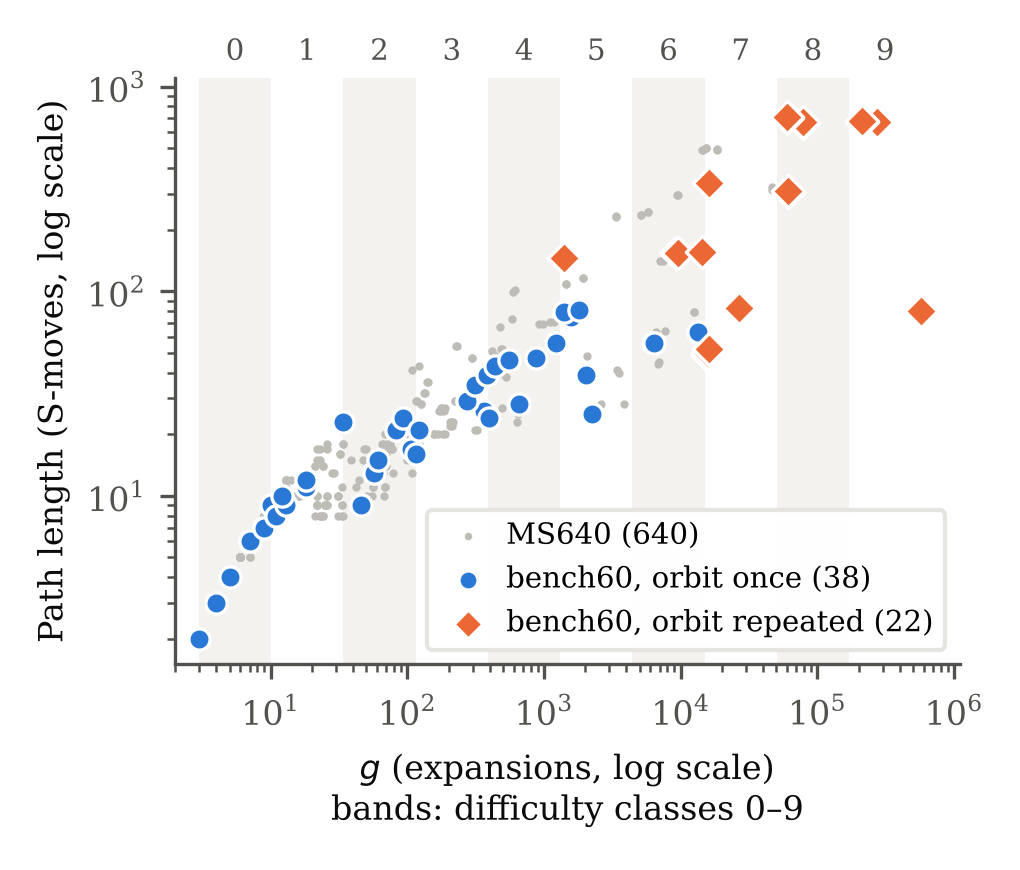
\includegraphics[width=0.49\textwidth]{figures/bench60_path.png}
\caption{bench60 inside MS640. Grey: all $640$ presentations; colour: the $60$ choices, six per difficulty class. Blue circles are choices whose
$\Aut(\F_2)$-orbit occurs once in bench60; diamonds are choices that share an orbit with another choice, which classes 7--9 force.
Left: $g$ against the rows sorted by $g$; the shaded bands are difficulty classes 0--9, each $3.37$ times the one below.
Right: the S-move length of a presentation against $g$.}
\label{fig:bench60}
\end{figure}

\subsection{ladder100}\label{app:ladder}

Each level of ladder100 (Definition~\ref{def:ladder}) contains $10$ presentations taken from AC19\_autmin and MS640;
Table~\ref{tab:ladder} gives the range of $g$ of each level. Here $g>10^7$ indicates that LENGTH fails within $10^7$
expansions, and $g_S$ denotes the number of expansions that $\SMK$ requires. At levels $1$--$6$ the presentations are
spread over the range of $g$ of the level, and at level $9$ over the range of $g_S$. Level $7$ takes the presentations
with the largest $g_S$, and level $8$ those with the largest $g$. Level $10$ consists of the presentations on which
$\SMK$ also fails within $10^7$ expansions.

Every presentation of ladder100 is AC-trivial. Those taken from MS640 are solved by LENGTH. For a presentation of
AC19\_autmin, the corresponding presentation of the extended AC19 data set is solved, and its S-moves are carried over to
the $\Aut(\F_2)$-minimal form.

\begin{table}[ht]
\centering
\begin{tabular}{rlrrrr}
\toprule
level & $g$ & from MS640 & mean $\lambda$ & mean $g$ & mean $g_S$\\
\midrule
1 & $<10^3$ & $5$ & $15.3$ & $214$ & $101$\\
2 & $10^3$--$10^4$ & $5$ & $19.9$ & $3{,}983$ & $707$\\
3 & $10^4$--$10^{4.5}$ & $5$ & $21.1$ & $17{,}612$ & $7{,}646$\\
4 & $10^{4.5}$--$10^5$ & $5$ & $21.5$ & $56{,}183$ & $9{,}780$\\
5 & $10^5$--$10^{5.5}$ & $4$ & $22.5$ & $235{,}756$ & $13{,}312$\\
6 & $10^{5.5}$--$10^6$ & $2$ & $19.4$ & $588{,}638$ & $4{,}693$\\
7 & $10^6$--$3\cdot10^6$ & $0$ & $20.2$ & $1{,}875{,}962$ & $424{,}977$\\
8 & $3\cdot10^6$--$10^7$ & $0$ & $18.8$ & $5{,}022{,}975$ & $113{,}309$\\
9 & $>10^7$ & $0$ & $21.0$ & -- & $340{,}650$\\
10$^{*}$ & $>10^7$ & $0$ & $18.3$ & -- & --\\
\bottomrule
\end{tabular}

\smallskip
{\small $^{*}$Only $9$ presentations fail for $\SMK$, so the tenth, \texttt{ac19\_12445}, is the next hardest one for
$\SMK$ from level $9$: it needs $1{,}297{,}772$ expansions.}
\caption{The levels of ladder100: the range of $g$, the number of the $10$ presentations taken from MS640 (the rest
are from AC19\_autmin), and the means of the starting total length $\lambda$, of $g$ and of $g_S$.}
\label{tab:ladder}
\end{table}

\subsection{Time per unit}\label{app:time}

An expansion performs different work in each method. LENGTH and $\SMK$ differ only in the priority they compute; the
hybrid additionally constructs the Nielsen images and runs the finishing checks; and a change of variables constructs
images of the state in place of S-move children. Equal budgets in units therefore constitute a fair comparison only
if a unit costs approximately the same in each method. To quantify the difference, one expansion of each method is
timed on the same states. For each test state, each method starts a fresh search, so that the heap holds only that
state, and performs one expansion: it removes the state, generates all of its children, discards those already
discovered, computes the priorities of the remainder and pushes them onto the heap. The test states are drawn at random
from the states that LENGTH and $\SMK$ expanded on MS640 with a budget of $10^4$ units, up to $60$ per range of total
length $\lambda$, and every method is timed on the same states. All methods run in pure Python (one core, Intel Xeon
$2.1$ GHz, best of five runs).
\begin{center}
\small
\begin{tabular}{lrrrrr}
\toprule
$\lambda$ & states & LENGTH & $\SMK$ & hybrid & CoV\\
\midrule
$\le10$ & $46$ & $0.12$ & $0.14$ & $0.28$ & $0.25$\\
$11$--$15$ & $60$ & $0.85$ & $1.05$ & $1.37$ & $3.24$\\
$16$--$20$ & $60$ & $1.61$ & $2.00$ & $3.03$ & $6.05$\\
$21$--$25$ & $60$ & $2.99$ & $3.41$ & $10.08$ & $11.23$\\
$\ge26$ & $60$ & $4.66$ & $6.00$ & $6.85$ & $16.47$\\
\midrule
mean & & $2.04$ & $2.52$ & $4.32$ & $7.45$\\
relative to LENGTH & & $1$ & $1.23$ & $2.11$ & $3.64$\\
\bottomrule
\end{tabular}

\smallskip
\footnotesize Time of one pop in ms, averaged over the states of the row. The mean row averages the five rows; the last row divides it by the LENGTH mean.
\end{center}
For example, one expansion of $\mathrm{AK}(3)$ ($\lambda=13$) takes $0.69$ ms for LENGTH, $0.87$ ms for $\SMK$,
$1.17$ ms for the hybrid and $2.61$ ms for the change of variables. A longer state has more children, so its expansion
costs more. An expansion of $\SMK$ differs from one of LENGTH only in its priority and costs $1.1$--$1.3$ times as much.
An expansion of the hybrid also constructs the four Nielsen images and runs the finishing checks, and costs $1.5$--$3.4$
times as much; its remaining units are single moves and cost less. Constructing the change-of-variables images of a
state costs $3.5$--$3.8$ expansions of LENGTH for $\lambda>10$. A unit of each method thus costs within a small factor
of one expansion of LENGTH, and equal budgets in units are comparable up to that factor.
; no preamble here.
% One big unnumbered section, "Appendix"; each part is a subsection lettered A, B, C, ...
% Add the next part as another \subsection{...}\label{app:...} below.
\section*{Appendix}\label{sec:appendix}
\addcontentsline{toc}{section}{Appendix}
\setcounter{subsection}{0}
\renewcommand{\thesubsection}{\Alph{subsection}}

\subsection{bench60}\label{app:bench60}

\begin{definition}[bench60, full rule]\label{def:bench60full}
Let $g_0=3$ and $g_{10}=574{,}959$ be the least and the largest value of $g$ on MS640 at budget $10^6$, and
let $\rho=(g_{10}/g_0)^{1/10}\approx3.37$. The \emph{difficulty class} $b\in\{0,\dots,9\}$ is the set of $P\in$ MS640 with
$g_0\rho^{b}\le g(P)<g_0\rho^{b+1}$ (class $9$ closed on the right). \textbf{bench60} takes $6$ presentations from every
difficulty class by the following rule.
\begin{enumerate}
  \item Over the whole subset, minimise the number of pairs of chosen presentations in the same $\Aut(\F_2)$-orbit.
  \item Subject to (1), sort the presentations of each difficulty class by path length, the number of S-moves in the solution GS-SUB finds; break ties by smaller $g$ first, then by line number in MS640.
  Take the $6$ presentations closest to $6$ evenly spaced positions of this sorted list, the first and the last
  position included.
  % This one needs more explaination
\end{enumerate}
\end{definition}

Figure~\ref{fig:bench60} shows where the $60$ rows lie in MS640.

\begin{center}
\begin{tabular}{rrrrr}
\toprule
class $b$ & range of $g$ & rows of MS640 & rows of bench60 & mean $g$ on bench60\\
\midrule
0 & $[3,\,11)$ & $317$ & $6$ & $6.3$\\
1 & $[11,\,35)$ & $89$ & $6$ & $17.7$\\
2 & $[35,\,116)$ & $63$ & $6$ & $74.3$\\
3 & $[116,\,390)$ & $60$ & $6$ & $261.7$\\
4 & $[390,\,1{,}314)$ & $31$ & $6$ & $691.2$\\
5 & $[1{,}314,\,4{,}433)$ & $26$ & $6$ & $1{,}746.8$\\
6 & $[4{,}433,\,14{,}959)$ & $28$ & $6$ & $9{,}869.2$\\
7 & $[14{,}959,\,50{,}482)$ & $14$ & $6$ & $19{,}596.3$\\
8 & $[50{,}482,\,170{,}367)$ & $6$ & $6$ & $66{,}530.7$\\
9 & $[170{,}367,\,574{,}959]$ & $6$ & $6$ & $353{,}647.7$\\
\midrule
all & & $640$ & $60$ & \\
\bottomrule
\end{tabular}
\end{center}

\begin{figure}[ht]
\centering
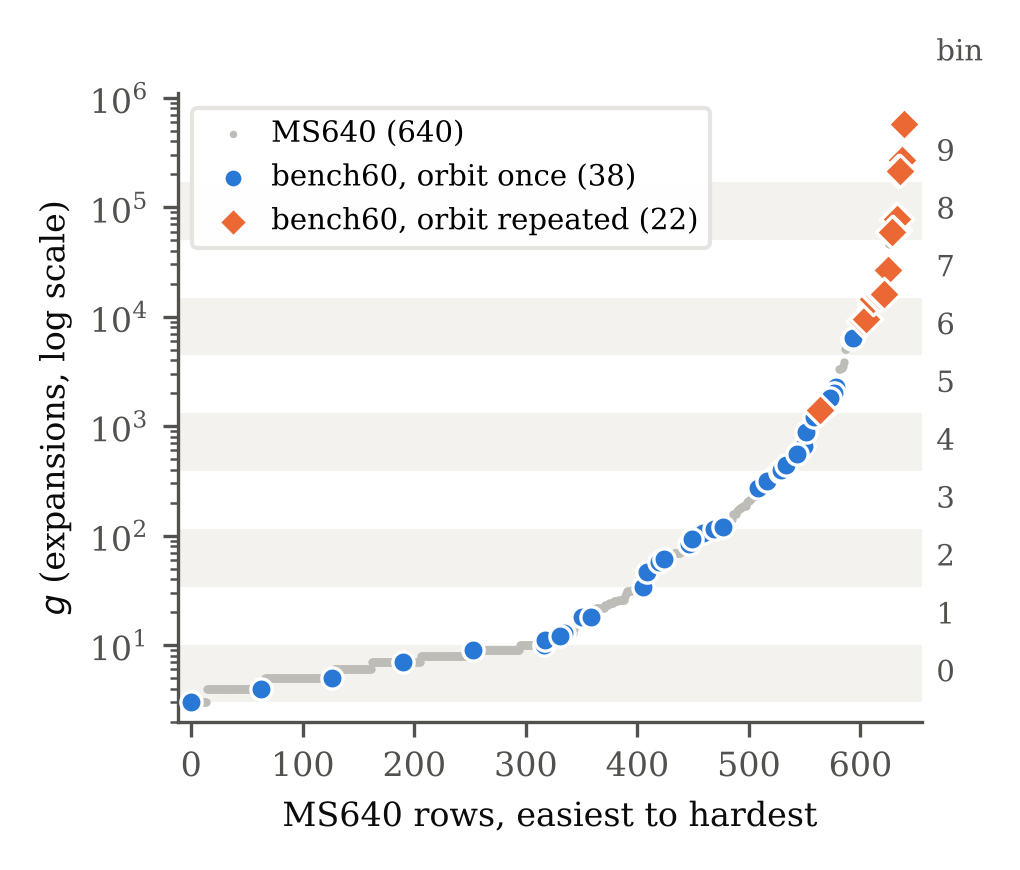
\includegraphics[width=0.49\textwidth]{figures/bench60_g.png}\hfill
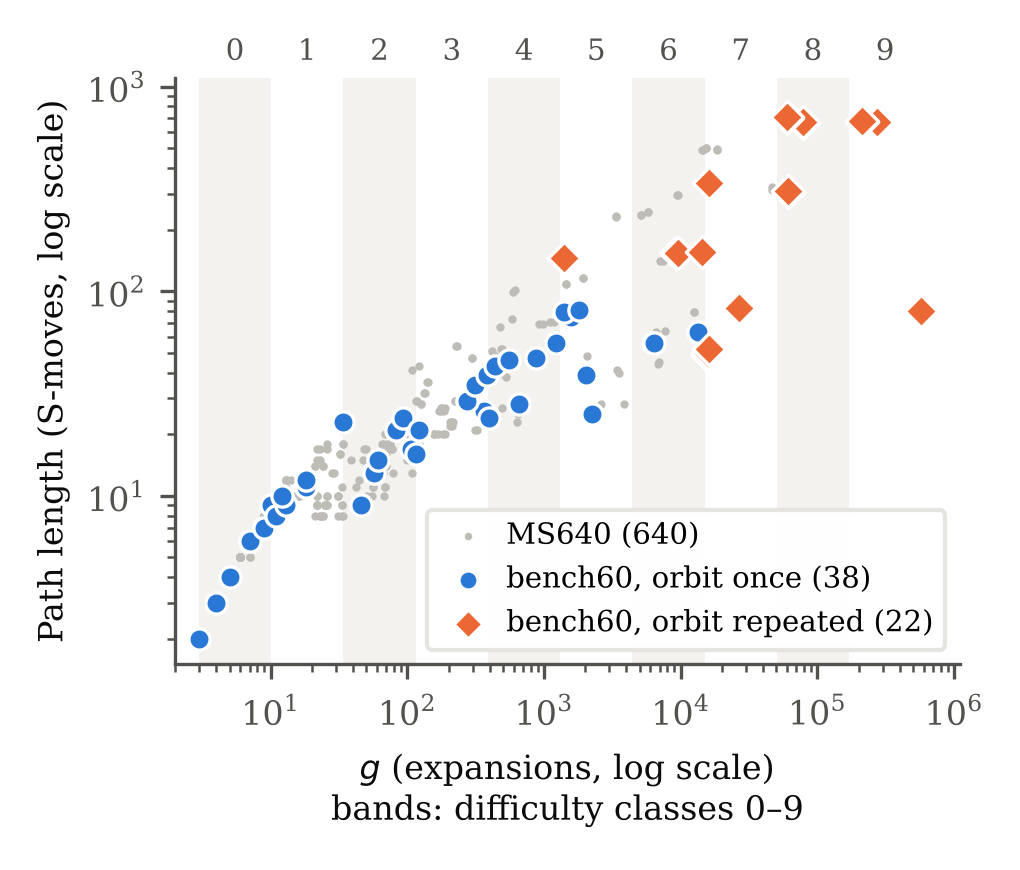
\includegraphics[width=0.49\textwidth]{figures/bench60_path.png}
\caption{bench60 inside MS640. Grey: all $640$ presentations; colour: the $60$ choices, six per difficulty class. Blue circles are choices whose
$\Aut(\F_2)$-orbit occurs once in bench60; diamonds are choices that share an orbit with another choice, which classes 7--9 force.
Left: $g$ against the rows sorted by $g$; the shaded bands are difficulty classes 0--9, each $3.37$ times the one below.
Right: the S-move length of a presentation against $g$.}
\label{fig:bench60}
\end{figure}

\subsection{ladder100}\label{app:ladder}

Each level of ladder100 (Definition~\ref{def:ladder}) contains $10$ presentations taken from AC19\_autmin and MS640;
Table~\ref{tab:ladder} gives the range of $g$ of each level. Here $g>10^7$ indicates that LENGTH fails within $10^7$
expansions, and $g_S$ denotes the number of expansions that $\SMK$ requires. At levels $1$--$6$ the presentations are
spread over the range of $g$ of the level, and at level $9$ over the range of $g_S$. Level $7$ takes the presentations
with the largest $g_S$, and level $8$ those with the largest $g$. Level $10$ consists of the presentations on which
$\SMK$ also fails within $10^7$ expansions.

Every presentation of ladder100 is AC-trivial. Those taken from MS640 are solved by LENGTH. For a presentation of
AC19\_autmin, the corresponding presentation of the extended AC19 data set is solved, and its S-moves are carried over to
the $\Aut(\F_2)$-minimal form.

\begin{table}[ht]
\centering
\begin{tabular}{rlrrrr}
\toprule
level & $g$ & from MS640 & mean $\lambda$ & mean $g$ & mean $g_S$\\
\midrule
1 & $<10^3$ & $5$ & $15.3$ & $214$ & $101$\\
2 & $10^3$--$10^4$ & $5$ & $19.9$ & $3{,}983$ & $707$\\
3 & $10^4$--$10^{4.5}$ & $5$ & $21.1$ & $17{,}612$ & $7{,}646$\\
4 & $10^{4.5}$--$10^5$ & $5$ & $21.5$ & $56{,}183$ & $9{,}780$\\
5 & $10^5$--$10^{5.5}$ & $4$ & $22.5$ & $235{,}756$ & $13{,}312$\\
6 & $10^{5.5}$--$10^6$ & $2$ & $19.4$ & $588{,}638$ & $4{,}693$\\
7 & $10^6$--$3\cdot10^6$ & $0$ & $20.2$ & $1{,}875{,}962$ & $424{,}977$\\
8 & $3\cdot10^6$--$10^7$ & $0$ & $18.8$ & $5{,}022{,}975$ & $113{,}309$\\
9 & $>10^7$ & $0$ & $21.0$ & -- & $340{,}650$\\
10$^{*}$ & $>10^7$ & $0$ & $18.3$ & -- & --\\
\bottomrule
\end{tabular}

\smallskip
{\small $^{*}$Only $9$ presentations fail for $\SMK$, so the tenth, \texttt{ac19\_12445}, is the next hardest one for
$\SMK$ from level $9$: it needs $1{,}297{,}772$ expansions.}
\caption{The levels of ladder100: the range of $g$, the number of the $10$ presentations taken from MS640 (the rest
are from AC19\_autmin), and the means of the starting total length $\lambda$, of $g$ and of $g_S$.}
\label{tab:ladder}
\end{table}

\subsection{Time per unit}\label{app:time}

An expansion performs different work in each method. LENGTH and $\SMK$ differ only in the priority they compute; the
hybrid additionally constructs the Nielsen images and runs the finishing checks; and a change of variables constructs
images of the state in place of S-move children. Equal budgets in units therefore constitute a fair comparison only
if a unit costs approximately the same in each method. To quantify the difference, one expansion of each method is
timed on the same states. For each test state, each method starts a fresh search, so that the heap holds only that
state, and performs one expansion: it removes the state, generates all of its children, discards those already
discovered, computes the priorities of the remainder and pushes them onto the heap. The test states are drawn at random
from the states that LENGTH and $\SMK$ expanded on MS640 with a budget of $10^4$ units, up to $60$ per range of total
length $\lambda$, and every method is timed on the same states. All methods run in pure Python (one core, Intel Xeon
$2.1$ GHz, best of five runs).
\begin{center}
\small
\begin{tabular}{lrrrrr}
\toprule
$\lambda$ & states & LENGTH & $\SMK$ & hybrid & CoV\\
\midrule
$\le10$ & $46$ & $0.12$ & $0.14$ & $0.28$ & $0.25$\\
$11$--$15$ & $60$ & $0.85$ & $1.05$ & $1.37$ & $3.24$\\
$16$--$20$ & $60$ & $1.61$ & $2.00$ & $3.03$ & $6.05$\\
$21$--$25$ & $60$ & $2.99$ & $3.41$ & $10.08$ & $11.23$\\
$\ge26$ & $60$ & $4.66$ & $6.00$ & $6.85$ & $16.47$\\
\midrule
mean & & $2.04$ & $2.52$ & $4.32$ & $7.45$\\
relative to LENGTH & & $1$ & $1.23$ & $2.11$ & $3.64$\\
\bottomrule
\end{tabular}

\smallskip
\footnotesize Time of one pop in ms, averaged over the states of the row. The mean row averages the five rows; the last row divides it by the LENGTH mean.
\end{center}
For example, one expansion of $\mathrm{AK}(3)$ ($\lambda=13$) takes $0.69$ ms for LENGTH, $0.87$ ms for $\SMK$,
$1.17$ ms for the hybrid and $2.61$ ms for the change of variables. A longer state has more children, so its expansion
costs more. An expansion of $\SMK$ differs from one of LENGTH only in its priority and costs $1.1$--$1.3$ times as much.
An expansion of the hybrid also constructs the four Nielsen images and runs the finishing checks, and costs $1.5$--$3.4$
times as much; its remaining units are single moves and cost less. Constructing the change-of-variables images of a
state costs $3.5$--$3.8$ expansions of LENGTH for $\lambda>10$. A unit of each method thus costs within a small factor
of one expansion of LENGTH, and equal budgets in units are comparable up to that factor.
; no preamble here.
% One big unnumbered section, "Appendix"; each part is a subsection lettered A, B, C, ...
% Add the next part as another \subsection{...}\label{app:...} below.
\section*{Appendix}\label{sec:appendix}
\addcontentsline{toc}{section}{Appendix}
\setcounter{subsection}{0}
\renewcommand{\thesubsection}{\Alph{subsection}}

\subsection{bench60}\label{app:bench60}

\begin{definition}[bench60, full rule]\label{def:bench60full}
Let $g_0=3$ and $g_{10}=574{,}959$ be the least and the largest value of $g$ on MS640 at budget $10^6$, and
let $\rho=(g_{10}/g_0)^{1/10}\approx3.37$. The \emph{difficulty class} $b\in\{0,\dots,9\}$ is the set of $P\in$ MS640 with
$g_0\rho^{b}\le g(P)<g_0\rho^{b+1}$ (class $9$ closed on the right). \textbf{bench60} takes $6$ presentations from every
difficulty class by the following rule.
\begin{enumerate}
  \item Over the whole subset, minimise the number of pairs of chosen presentations in the same $\Aut(\F_2)$-orbit.
  \item Subject to (1), sort the presentations of each difficulty class by path length, the number of S-moves in the solution GS-SUB finds; break ties by smaller $g$ first, then by line number in MS640.
  Take the $6$ presentations closest to $6$ evenly spaced positions of this sorted list, the first and the last
  position included.
  % This one needs more explaination
\end{enumerate}
\end{definition}

Figure~\ref{fig:bench60} shows where the $60$ rows lie in MS640.

\begin{center}
\begin{tabular}{rrrrr}
\toprule
class $b$ & range of $g$ & rows of MS640 & rows of bench60 & mean $g$ on bench60\\
\midrule
0 & $[3,\,11)$ & $317$ & $6$ & $6.3$\\
1 & $[11,\,35)$ & $89$ & $6$ & $17.7$\\
2 & $[35,\,116)$ & $63$ & $6$ & $74.3$\\
3 & $[116,\,390)$ & $60$ & $6$ & $261.7$\\
4 & $[390,\,1{,}314)$ & $31$ & $6$ & $691.2$\\
5 & $[1{,}314,\,4{,}433)$ & $26$ & $6$ & $1{,}746.8$\\
6 & $[4{,}433,\,14{,}959)$ & $28$ & $6$ & $9{,}869.2$\\
7 & $[14{,}959,\,50{,}482)$ & $14$ & $6$ & $19{,}596.3$\\
8 & $[50{,}482,\,170{,}367)$ & $6$ & $6$ & $66{,}530.7$\\
9 & $[170{,}367,\,574{,}959]$ & $6$ & $6$ & $353{,}647.7$\\
\midrule
all & & $640$ & $60$ & \\
\bottomrule
\end{tabular}
\end{center}

\begin{figure}[ht]
\centering
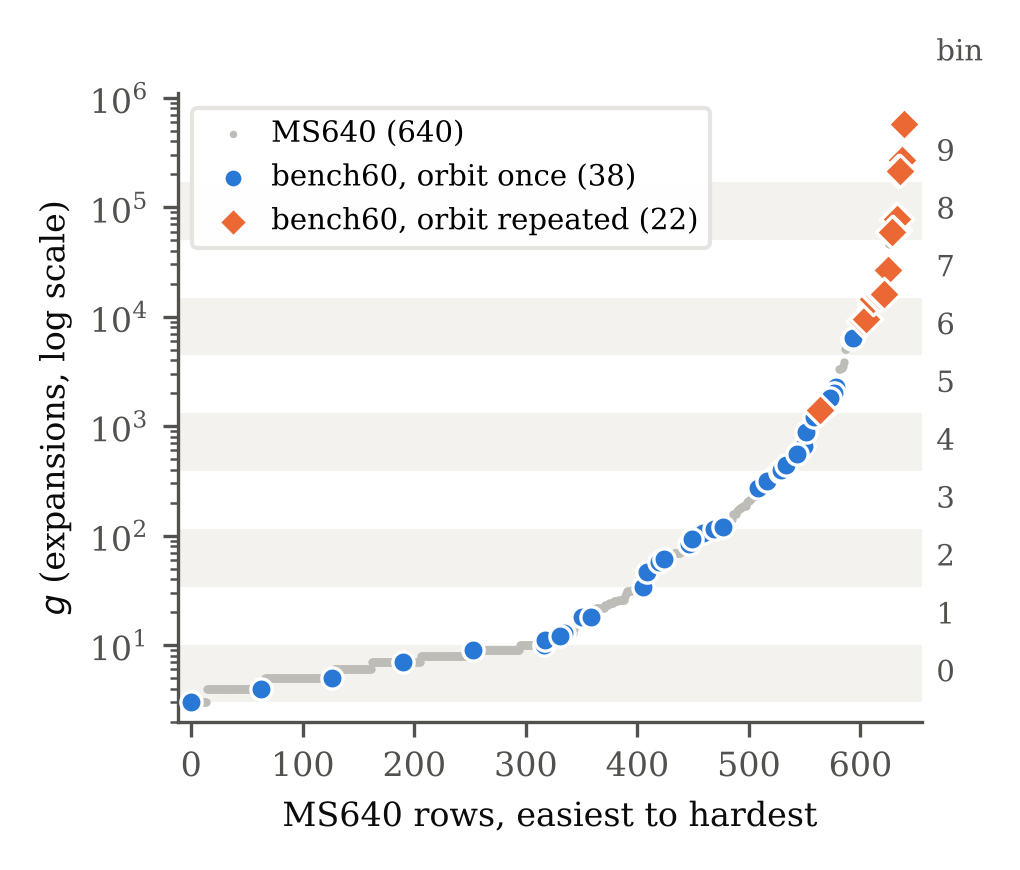
\includegraphics[width=0.49\textwidth]{figures/bench60_g.png}\hfill
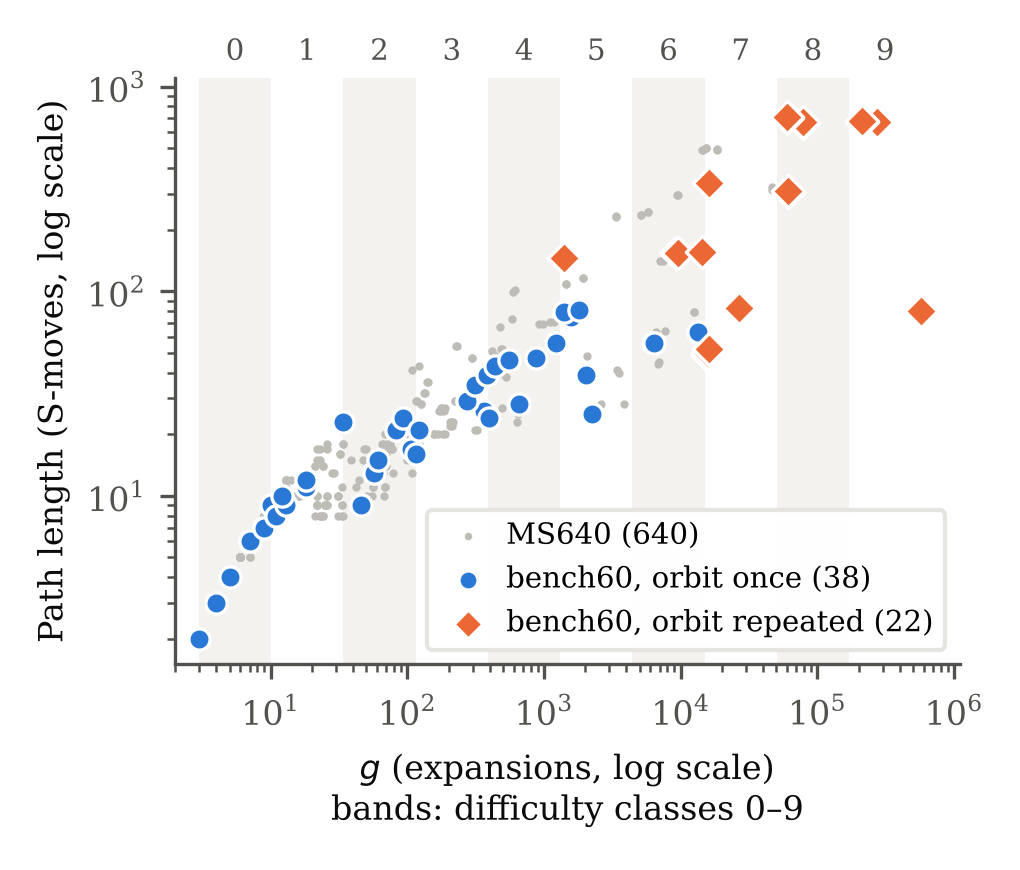
\includegraphics[width=0.49\textwidth]{figures/bench60_path.png}
\caption{bench60 inside MS640. Grey: all $640$ presentations; colour: the $60$ choices, six per difficulty class. Blue circles are choices whose
$\Aut(\F_2)$-orbit occurs once in bench60; diamonds are choices that share an orbit with another choice, which classes 7--9 force.
Left: $g$ against the rows sorted by $g$; the shaded bands are difficulty classes 0--9, each $3.37$ times the one below.
Right: the S-move length of a presentation against $g$.}
\label{fig:bench60}
\end{figure}

\subsection{ladder100}\label{app:ladder}

Each level of ladder100 (Definition~\ref{def:ladder}) contains $10$ presentations taken from AC19\_autmin and MS640;
Table~\ref{tab:ladder} gives the range of $g$ of each level. Here $g>10^7$ indicates that LENGTH fails within $10^7$
expansions, and $g_S$ denotes the number of expansions that $\SMK$ requires. At levels $1$--$6$ the presentations are
spread over the range of $g$ of the level, and at level $9$ over the range of $g_S$. Level $7$ takes the presentations
with the largest $g_S$, and level $8$ those with the largest $g$. Level $10$ consists of the presentations on which
$\SMK$ also fails within $10^7$ expansions.

Every presentation of ladder100 is AC-trivial. Those taken from MS640 are solved by LENGTH. For a presentation of
AC19\_autmin, the corresponding presentation of the extended AC19 data set is solved, and its S-moves are carried over to
the $\Aut(\F_2)$-minimal form.

\begin{table}[ht]
\centering
\begin{tabular}{rlrrrr}
\toprule
level & $g$ & from MS640 & mean $\lambda$ & mean $g$ & mean $g_S$\\
\midrule
1 & $<10^3$ & $5$ & $15.3$ & $214$ & $101$\\
2 & $10^3$--$10^4$ & $5$ & $19.9$ & $3{,}983$ & $707$\\
3 & $10^4$--$10^{4.5}$ & $5$ & $21.1$ & $17{,}612$ & $7{,}646$\\
4 & $10^{4.5}$--$10^5$ & $5$ & $21.5$ & $56{,}183$ & $9{,}780$\\
5 & $10^5$--$10^{5.5}$ & $4$ & $22.5$ & $235{,}756$ & $13{,}312$\\
6 & $10^{5.5}$--$10^6$ & $2$ & $19.4$ & $588{,}638$ & $4{,}693$\\
7 & $10^6$--$3\cdot10^6$ & $0$ & $20.2$ & $1{,}875{,}962$ & $424{,}977$\\
8 & $3\cdot10^6$--$10^7$ & $0$ & $18.8$ & $5{,}022{,}975$ & $113{,}309$\\
9 & $>10^7$ & $0$ & $21.0$ & -- & $340{,}650$\\
10$^{*}$ & $>10^7$ & $0$ & $18.3$ & -- & --\\
\bottomrule
\end{tabular}

\smallskip
{\small $^{*}$Only $9$ presentations fail for $\SMK$, so the tenth, \texttt{ac19\_12445}, is the next hardest one for
$\SMK$ from level $9$: it needs $1{,}297{,}772$ expansions.}
\caption{The levels of ladder100: the range of $g$, the number of the $10$ presentations taken from MS640 (the rest
are from AC19\_autmin), and the means of the starting total length $\lambda$, of $g$ and of $g_S$.}
\label{tab:ladder}
\end{table}

\subsection{Time per unit}\label{app:time}

An expansion performs different work in each method. LENGTH and $\SMK$ differ only in the priority they compute; the
hybrid additionally constructs the Nielsen images and runs the finishing checks; and a change of variables constructs
images of the state in place of S-move children. Equal budgets in units therefore constitute a fair comparison only
if a unit costs approximately the same in each method. To quantify the difference, one expansion of each method is
timed on the same states. For each test state, each method starts a fresh search, so that the heap holds only that
state, and performs one expansion: it removes the state, generates all of its children, discards those already
discovered, computes the priorities of the remainder and pushes them onto the heap. The test states are drawn at random
from the states that LENGTH and $\SMK$ expanded on MS640 with a budget of $10^4$ units, up to $60$ per range of total
length $\lambda$, and every method is timed on the same states. All methods run in pure Python (one core, Intel Xeon
$2.1$ GHz, best of five runs).
\begin{center}
\small
\begin{tabular}{lrrrrr}
\toprule
$\lambda$ & states & LENGTH & $\SMK$ & hybrid & CoV\\
\midrule
$\le10$ & $46$ & $0.12$ & $0.14$ & $0.28$ & $0.25$\\
$11$--$15$ & $60$ & $0.85$ & $1.05$ & $1.37$ & $3.24$\\
$16$--$20$ & $60$ & $1.61$ & $2.00$ & $3.03$ & $6.05$\\
$21$--$25$ & $60$ & $2.99$ & $3.41$ & $10.08$ & $11.23$\\
$\ge26$ & $60$ & $4.66$ & $6.00$ & $6.85$ & $16.47$\\
\midrule
mean & & $2.04$ & $2.52$ & $4.32$ & $7.45$\\
relative to LENGTH & & $1$ & $1.23$ & $2.11$ & $3.64$\\
\bottomrule
\end{tabular}

\smallskip
\footnotesize Time of one pop in ms, averaged over the states of the row. The mean row averages the five rows; the last row divides it by the LENGTH mean.
\end{center}
For example, one expansion of $\mathrm{AK}(3)$ ($\lambda=13$) takes $0.69$ ms for LENGTH, $0.87$ ms for $\SMK$,
$1.17$ ms for the hybrid and $2.61$ ms for the change of variables. A longer state has more children, so its expansion
costs more. An expansion of $\SMK$ differs from one of LENGTH only in its priority and costs $1.1$--$1.3$ times as much.
An expansion of the hybrid also constructs the four Nielsen images and runs the finishing checks, and costs $1.5$--$3.4$
times as much; its remaining units are single moves and cost less. Constructing the change-of-variables images of a
state costs $3.5$--$3.8$ expansions of LENGTH for $\lambda>10$. A unit of each method thus costs within a small factor
of one expansion of LENGTH, and equal budgets in units are comparable up to that factor.


\end{document}
